% !TeX program = xelatex
\documentclass[]{IAC_style}

% English manuscript. Compile with XeLaTeX.
% IAC_style provides the Times-compatible newtx mathematics.
\usepackage{amsmath}
% Use one consistent row spacing for all multi-line display equations.
\setlength{\jot}{4pt}
\usepackage{enumitem}
\usepackage{subcaption}
\usepackage{array}
\usepackage{microtype}
\usepackage{placeins}
\usepackage{float}
\usepackage{tikz}
\usetikzlibrary{arrows.meta,fit,positioning}
\graphicspath{{pics/}{pics/docx/}}

\newcommand{\imageplaceholder}[2][3.1cm]{%
  \fbox{\parbox[c][#1][c]{0.92\linewidth}{\centering\footnotesize #2}}%
}
\newcommand{\placeholderfigure}[2]{%
  \begin{figure}[t]
  \centering
  \imageplaceholder{#2}
  \caption{#1}
  \end{figure}
}

\begin{document}

\IACpaperyear{2026}
\IACpapernumber{IAC-26,C1,5,6,x108402}
\IACconference{77th International Astronautical Congress (IAC 2026)}
\IAClocation{Antalya, T\"urkiye}
\IACdate{5--9 Oct 2026}
\IACcopyrightA{}

\title{Development and Verification of a Multisensor Navigation System Using an Error-State Kalman Filter for Lunar Rovers}

% Author and affiliation information from the KSAS 2025 Fall Conference paper.
\IACauthor{Chulsoo Lim}{1}{0}
\IACauthor{Hosun Lee}{1}{0}
\IACauthor{Soohyeok Choi}{2}{0}
\IACauthor{Dongyoung Kwon}{3}{0}
\IACauthor{Sunwook Kim}{3}{0}
\IACauthor{Kicheol Jeong}{3}{0}
\IACauthor{Hyomin Jin}{3}{0}
\IACauthor{Kyudong Kim}{3}{0}
\IACauthor{Hyeonil Lee}{3}{0}
\IACauthor{Youngseok Lee}{3}{0}
\IACauthor{Gihan Noh}{3}{0}
\IACauthor{Hyungsic Park}{4}{0}
\IACauthor{Mangyu Lee}{4}{0}
\IACauthor{Junhwi Cho}{4}{0}
\IACauthor{Kwangwoo Jang}{5}{0}
\IACauthor{Junwoo Park}{1}{0}
\IACauthor{Hohyeong Lee}{1}{0}
\IACauthor{Hyo Choong Bang}{1}{1}
\IACauthoraffiliation{Department of Aerospace Engineering, Korea Advanced Institute of Science and Technology (KAIST), 291 Daehak-ro, Yuseong-gu, Daejeon 34141, Republic of Korea. \normalfont{Email addresses:~\authormail{charleslim@kaist.ac.kr} (C. Lim); \authormail{hcbang@kaist.ac.kr} (H.C. Bang, corresponding author).}}
\IACauthoraffiliation{Nmotion, Incheon, Republic of Korea. / Department of Automotive Engineering, Hanyang University, Seoul 04763, Republic of Korea.}
\IACauthoraffiliation{Korea Automotive Technology Institute (KATECH), Cheonan 31214, Republic of Korea.}
\IACauthoraffiliation{Hyundai Motor Company, Seoul 06797, Republic of Korea.}
\IACauthoraffiliation{Electronics and Telecommunications Research Institute, Daejeon 34129, Republic of Korea.}

\abstract{This study proposes a local navigation architecture based on an error-state Kalman filter (ESKF). The architecture integrates a fine Sun sensor (FSS), an inertial navigation system (INS), and wheel odometry for four independently steered wheels to support lunar surface operations when visual navigation is degraded or unavailable. The navigation state is propagated in a local Cartesian frame aligned with the initial direction of travel. Constant gravity and a locally planar surface are assumed for operation over short ranges and at low speeds. The proposed algorithm is verified progressively using a Microsoft AirSim/Unreal Engine simulation environment and hardware experiments with a full-scale rover. A gravity compensation device based on helium buoyancy reduces the effective normal load between the wheels and terrain during the ground tests to approximately one sixth of its terrestrial value. Across the four reported hardware position trials, the mean terminal horizontal position error normalized by the measured displacement was 4.5\% (mean Euclidean endpoint error: 0.20~m), while the mean absolute heading error across three heading trials was 0.26$^\circ$. The results demonstrate the feasibility of the real-time multisensor navigation framework and its recovery procedure for wheel contact disturbances.}

\IACkeywords{lunar rover navigation; error-state Kalman filter; fine Sun sensor; inertial navigation; wheel odometry; multisensor fusion.}

\maketitle
\thispagestyle{fancy}

\section*{Nomenclature and Abbreviations}
\begin{tabular}{@{}ll@{}}
ESKF & error-state Kalman filter \\
FSS & fine Sun sensor \\
INS & inertial navigation system \\
IMU & inertial measurement unit \\
VO & visual odometry \\
\end{tabular}

\section{Introduction}

International and commercial interest in lunar exploration has intensified through programs such as Artemis and Commercial Lunar Payload Services (CLPS). As a result, surface mobility has become a central topic in planetary robotics. Lunar rovers are being developed for cargo transport, scientific exploration, and in situ resource utilization. Reliable positioning and precise navigation are essential if these systems are to operate autonomously with limited support from Earth.

Unlike terrestrial autonomous vehicles, lunar rovers cannot use GNSS, high-accuracy terrestrial beacons, or a useful planetary magnetic field~\cite{ilyas2016integrated}. State estimation is therefore restricted to a small set of self-contained measurements, including inertial data, celestial observations, and wheel odometry. Their error characteristics must be modeled carefully and fused consistently.

The INS is a core element of a lunar rover navigation architecture because it provides high-bandwidth attitude, velocity, and position estimates without external infrastructure. When operated alone, however, the integration of bias and noise causes the navigation error to grow without bound. This effect is particularly significant for low-cost MEMS sensors. Periodic correction with at least one bounded absolute measurement is therefore required~\cite{titterton2004strapdown,groves2013principles}.

Previous Mars and lunar rovers have addressed this limitation using several aiding sensors. The Mars Exploration Rovers, Mars Science Laboratory, and Perseverance rely strongly on visual odometry (VO) and stereo terrain-relative navigation~\cite{maimone2007mer,rankin2021curiosity,maki2020mars2020}. The Chang'e/Yutu rovers combine inertial measurements, wheel odometry, and image-based localization~\cite{ma2020yutu2}. These missions demonstrate the maturity of visual navigation for planetary surface vehicles.

The performance and availability of VO depend on scene texture and illumination. Low-texture regolith, long shadows at low solar elevation, high contrast, temporary camera degradation, and limited onboard computing resources can reduce feature detection and matching reliability. A navigation aid independent of terrain imagery is therefore valuable as a complementary channel that improves system availability and fault tolerance.

\FloatBarrier
\begin{table*}[!t]
\centering
\caption{Representative navigation approaches used by planetary surface vehicles.}
\label{tab:rover_navigation}
\scriptsize
\begin{tabularx}{\textwidth}{p{0.13\textwidth}p{0.14\textwidth}p{0.30\textwidth}X}
\toprule
\textbf{Mission} & \textbf{Operation} & \textbf{Main Navigation Sensors} & \textbf{Navigation Approach} \\
\midrule
Apollo LRV~\cite{smith1973lrv} & Crew operated & Directional gyro, wheel odometers, Sun shadow device & Dead reckoning with solar heading check \\
MER Spirit / Opportunity~\cite{maimone2007mer} & Ground commands + AutoNav & Stereo cameras, IMU, wheel encoders & VO, terrain mapping, and slip compensation \\
MSL Curiosity~\cite{rankin2021curiosity} & Ground commands + AutoNav & Stereo cameras, IMU, wheel encoders & VO and terrain hazard assessment \\
Mars 2020 Perseverance~\cite{verma2023perseverance} & Enhanced AutoNav & Stereo cameras, IMU, wheel encoders & Continuous VO, mapping, and path planning \\
Chang'e-4 / Yutu-2~\cite{ma2020yutu2} & Ground in the loop & Stereo cameras, IMU, wheel odometry & Stereo mapping and rover localization \\
Chandrayaan-3 / Pragyan~\cite{isro2024pragyan} & Semi-autonomous & Stereo Navcams, mobility telemetry & Ground-generated DEM and path planning \\
SLIM / LEV-2~\cite{jaxa2024lev2} & Fully autonomous, short range & Dual cameras, onboard control & Autonomous mobility and imaging \\
IM-2 / YAOKI~\cite{dymon2025yaoki} & Teleoperated checkout & Camera, wheel telemetry & Images returned; not deployed or traversed \\
Rashid-1 / Rashid-2~\cite{ispace2023m1,mbrsc2026rashid} & Not deployed / planned & Navigation cameras, mobility sensors & No Rashid-1 surface operation; Rashid-2 mobility planned \\
Proposed system & Fallback mode without vision & FSS, IMU, wheel encoders & Local dead reckoning aided by FSS attitude and wheel odometry \\
\bottomrule
\end{tabularx}
\end{table*}

Celestial navigation based on Sun vector measurements has been studied as such an aid. Comparing a measured solar line-of-sight vector with the direction predicted from an onboard ephemeris and clock provides bounded absolute heading and inclination information~\cite{ilyas2016integrated,rhee2007satellite}. A Sun sensor is mechanically simple, radiation tolerant, and largely independent of terrain conditions, making it suitable for extended lunar operations.

The ESKF is a standard framework for fusing inertial, celestial, and odometric measurements~\cite{lefferts1982kalman,sola2017quaternion,sveinsson2012insgps,groves2013principles}. It tracks a small linearized error state around a nonlinearly propagated nominal state, handles the quaternion unit norm constraint consistently, and estimates attitude errors and IMU biases in minimal coordinates. These properties are well suited to lunar navigation with intermittent absolute updates.

This study implements and verifies a complete multisensor navigation system based on an ESKF for lunar rover operation. It evaluates whether a quaternion attitude correction constructed from the measured three-axis FSS Sun vector can bound INS attitude drift and whether wheel odometry can maintain local position continuity over short ranges when VO is unavailable or unreliable, provided that the Sun remains within the sensor field of view. The architecture combines an INS, a CMOS FSS, and wheel odometry from a rover with four independently steered wheels in one error state filter under assumptions of a local plane and constant gravity.

The main contributions are as follows.

\begin{enumerate}[label=(\roman*)]
\item A nonvisual local navigation architecture for a lunar rover that combines an INS, FSS, and wheel odometry for four independently steered wheels in a single ESKF. The measured three-axis Sun vector is aligned with its ephemeris prediction to form a minimum-rotation correction quaternion for the attitude update, while wheel odometry estimates velocity and displacement over short ranges. The rover kinematics support Ackermann steering, zero turns, and independent steering.

\item Simulation and real-time implementation of the integrated navigation algorithm. The ESKF is evaluated in a lunar surface environment based on Microsoft AirSim and Unreal Engine over straight, turning, slope, and composite route manoeuvres that include wheel slip intervals. The same algorithm is implemented on a NAVCOM comprising a Jetson Orin Nano and STM32F7 and checked through PILS and HILS.

\item Experimental verification of the wheel and inertial subsystem using a full-scale rover with four independently steered wheels and a gravity offloading system based on helium buoyancy. Indoor experiments focus on the IMU, wheel encoders, rover kinematics, and real-time NAVCOM implementation because the solar illumination geometry required for an FSS update cannot be reproduced faithfully indoors.
\end{enumerate}

Section 2 presents the navigation architecture and reference frames. Section 3 describes the local frame INS mechanization. Sections 4 and 5 develop the FSS and wheel odometry measurement models. Section 6 formulates the ESKF. Section 7 presents the simulation study, Section 8 presents the hardware tests, and Section 9 concludes the paper.

\section{Navigation Architecture and Reference Frames}

\subsection{Overall Navigation Architecture}

The sensor fusion concept is shown in Fig.~\ref{fig:navigation_overview}. A strapdown INS propagates attitude, velocity, and position at high rate using IMU angular rate and specific force measurements. The FSS channel transforms the measured three-axis Sun line-of-sight vector into the body frame and aligns it with the direction predicted from the onboard clock and ephemeris. The resulting correction quaternion is supplied to the ESKF as an attitude observation. The wheel encoders provide body frame velocity and yaw rate observations through the four-wheel kinematic model. The ESKF tracks the linearized errors of the nominal INS state and uses the aiding measurements to correct long-term drift. A monitoring and recovery channel rejects abnormal wheel measurements and reinitializes filter information when disturbances caused by pits or impacts between the wheels and terrain exceed the normal range.

\begin{figure*}[!t]
\centering
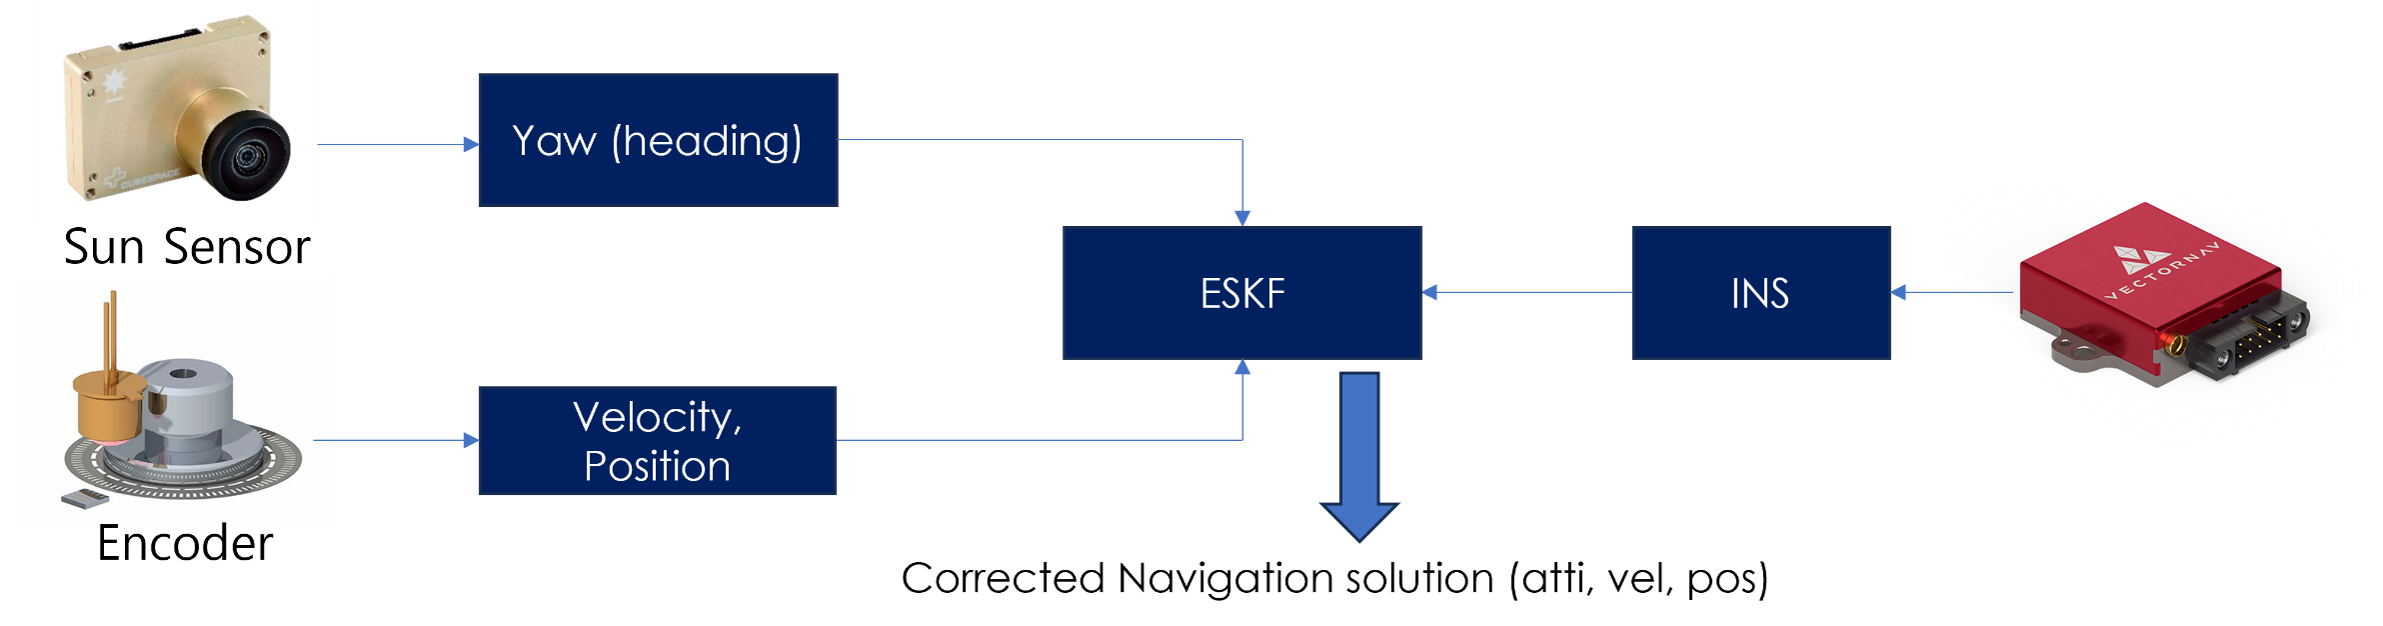
\includegraphics[width=0.96\textwidth]{pics/overview.png}
\caption{Overview of the ESKF navigation architecture integrating the FSS, IMU, and wheel odometry.}
\label{fig:navigation_overview}
\end{figure*}

The INS runs at the 200-Hz IMU sampling rate. FSS updates are processed asynchronously whenever a valid Sun image is acquired, typically at several hertz. Wheel encoders are sampled at the motor controller rate. Each asynchronous measurement invokes the corresponding ESKF update without changing the high-rate propagation loop.

The detailed software flow, including high-rate propagation and asynchronous measurement updates, is shown in Fig.~\ref{fig:navigation_sw_flow}.

\begin{figure*}[!t]
\centering
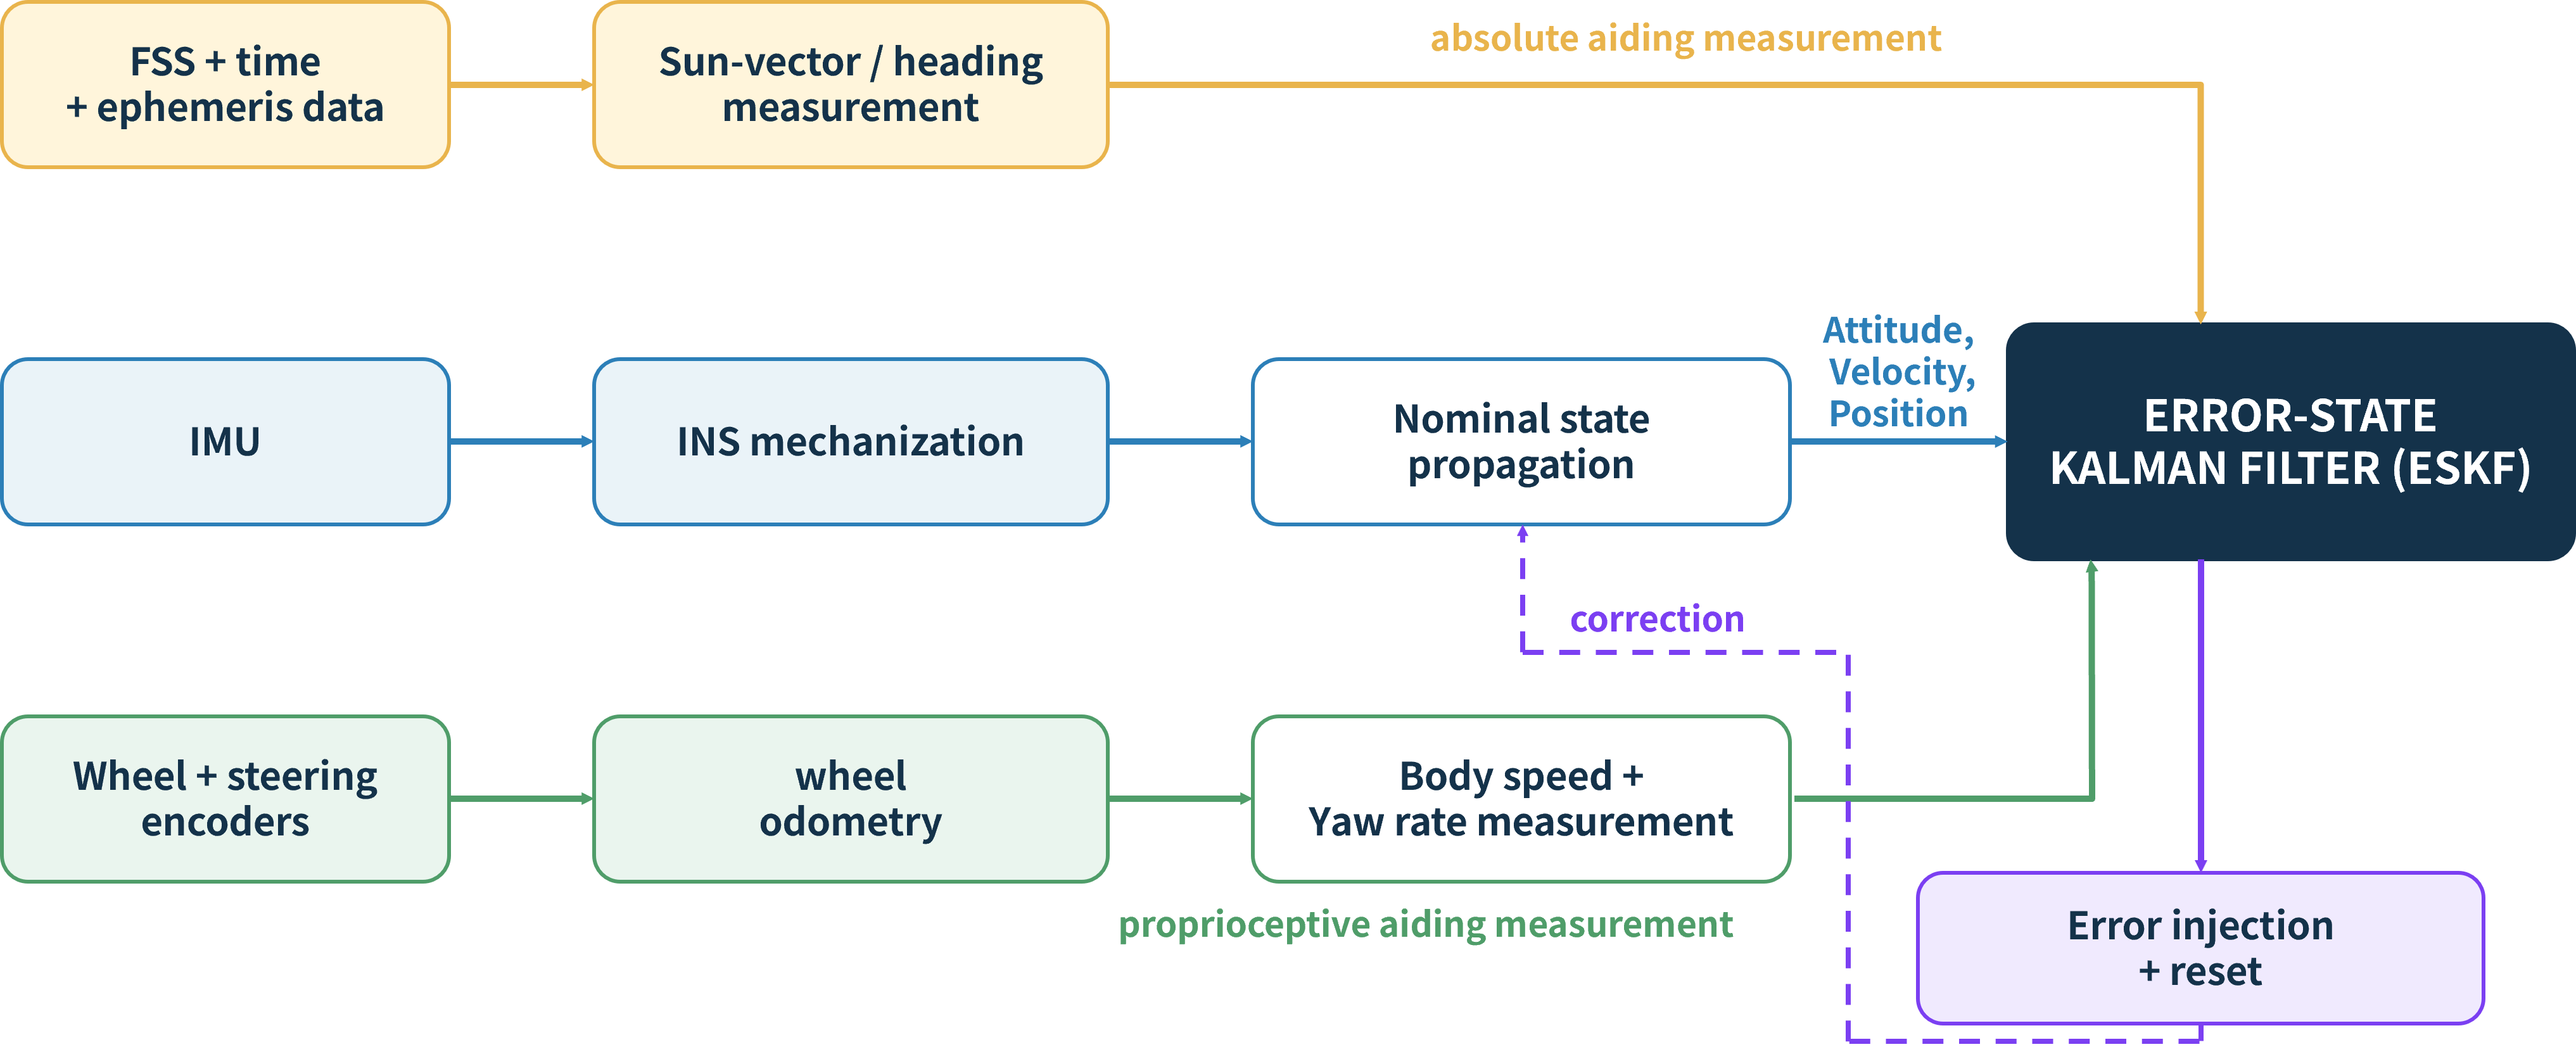
\includegraphics[width=0.98\textwidth]{pics/architecture.png}
\caption{High-rate propagation and asynchronous measurement update flow of the multisensor navigation software.}
\label{fig:navigation_sw_flow}
\end{figure*}

\subsection{Reference Frames and Notation}

The following right-handed orthonormal frames are used.
\begin{itemize}[leftmargin=*]
\item \textbf{Body frame $b$:} rover-fixed frame with its origin at the IMU. The $x_b$-axis points forward, $y_b$ to the right, and $z_b$ downward.
\item \textbf{Local navigation frame $\ell$:} local Cartesian frame fixed at the test starting point. The $x_\ell$-axis is aligned with the initial forward direction, $y_\ell$ points initially rightward, and $z_\ell$ points downward. Initially, $C_b^\ell(0)=I$.
\item \textbf{Sun sensor frame $\mathrm{ss}$:} frame fixed to the FSS housing, with $x_{\mathrm{ss}}$ along the optical axis. The fixed mounting alignment from the sensor frame to the body frame is $C_{\mathrm{ss}}^b$.
\end{itemize}

A rotation between frames is represented by a direction cosine matrix $C_a^b$ or quaternion $q_a^b$. The matrix transforms a vector expressed in frame $a$ into frame $b$:
\begin{equation*}
v^b=C_a^b v^a.
\end{equation*}
Rover position and velocity in the local frame are
\begin{equation*}
p^\ell=\begin{bmatrix}x&y&z\end{bmatrix}^{\top},\qquad v^\ell=\begin{bmatrix}v_x&v_y&v_z\end{bmatrix}^{\top}.
\end{equation*}
The navigation state is relative to the starting point rather than global lunar latitude, longitude, and altitude.

\subsection{Sensor Configuration}

Table~\ref{tab:sensors} summarizes the main sensor parameters. The IMU and motor encoders are integrated with the onboard navigation computer, and three FSS units are installed on the rover. For readability, Sec.~4 presents the measurement model for a generic FSS channel and omits the sensor index; the calibrated mounting matrix of FSS $j$ can be written as $C_{\mathrm{ss},j}^b$ when the individual channels must be distinguished.

\begin{table}[t]
\centering
\caption{Main sensor configuration of the test platform.}
\label{tab:sensors}
\scriptsize
\begin{tabularx}{\columnwidth}{p{0.19\columnwidth}p{0.29\columnwidth}X}
\toprule
\textbf{Sensor} & \textbf{Parameter} & \textbf{Value} \\
\midrule
IMU & Sampling rate & 200 Hz \\
 & Gyro bias & 10 deg/h class \\
 & Accelerometer bias & 1 mg class \\
FSS & Accuracy & 0.2 deg ($2\sigma$) \\
 & Number of units & Three \\
 & Field of view & 176 deg \\
 & Mass and power & 15 g, 100--174 mW \\
Encoders & Drive/steering channels & Four each \\
\bottomrule
\end{tabularx}
\end{table}

\section{Local Frame INS Mechanization}

The strapdown INS integrates IMU angular rate and specific force to propagate rover attitude, velocity, and position in the local frame $\ell$~\cite{titterton2004strapdown,groves2013principles}. The experiments are limited to short-range, low-speed motion. The lunar surface over the test area is approximated as a local plane with constant gravity. Lunar rotation, surface curvature, position-dependent gravity, and transport rate are neglected. This approximation is justified when $D/R_M\ll1$ and $\lVert 2\omega_M^\ell\times v^\ell\rVert$ is much smaller than the IMU error level, where $D$ is the maximum traverse distance, $R_M$ is the mean lunar radius, and $\omega_M^\ell$ is the lunar rotation vector expressed in the local frame, with $\lVert\omega_M^\ell\rVert\approx2.6617\times10^{-6}$~rad/s.

\subsection{Constant Gravity and Local Plane Assumptions}

Because $z_\ell$ points downward, the gravity vector is
\begin{equation}
\tag{1}\label{eq:1}
g^\ell=\begin{bmatrix}0&0&g_0\end{bmatrix}^{\top}.
\end{equation}
Here, $g_0$ is the effective gravitational acceleration used in the test environment. The configured lunar value is used in software simulation, while terrestrial tests compensate gravity according to the actual IMU environment. The helium buoyancy system changes the effective vertical wheel load but does not transform the terrestrial gravity field acting on the IMU into lunar gravity.

\subsection{Attitude Kinematics}

The attitude from the body frame to the local frame is represented by the unit quaternion
\begin{equation*}
q_b^\ell=\begin{bmatrix}q_w&q_x&q_y&q_z\end{bmatrix}^{\top}.
\end{equation*}
The bias-corrected gyro rate is
\begin{equation}
\tag{2}\label{eq:2}
\hat{\omega}_{\ell b}^b=\omega_m^b-b_g,
\end{equation}
where $\omega_m^b$ is the gyro measurement and $b_g$ is the estimated bias. With the local frame treated as inertially fixed during the test,
\begin{equation}
\tag{3}\label{eq:3}
\dot q_b^\ell=\frac{1}{2}q_b^\ell\otimes\begin{bmatrix}0\\\hat{\omega}_{\ell b}^b\end{bmatrix}.
\end{equation}
The symbol $\otimes$ denotes Hamilton quaternion multiplication. The quaternion is normalized after numerical integration.

\subsection{Velocity Update}

The bias-corrected specific force is $\hat f^b=f_m^b-b_a$, where $f_m^b$ is the accelerometer measurement and $b_a$ is the estimated accelerometer bias. The velocity equation is
\begin{equation}
\tag{4}\label{eq:4}
\dot v^\ell=C_b^\ell\left(f_m^b-b_a\right)+g^\ell.
\end{equation}
Coriolis and centrifugal acceleration, transport acceleration, and position-dependent gravity are omitted because they are small compared with bias and wheel slip errors over the test range.

\subsection{Position Update}

The local Cartesian position satisfies
\begin{equation}
\tag{5}\label{eq:5}
\dot p^\ell=v^\ell.
\end{equation}
Assuming constant acceleration over the IMU interval $\Delta t$,
\begin{equation}
\tag{6}\label{eq:6}
\begin{aligned}
p_{k+1}^\ell
  &=p_k^\ell+v_k^\ell\Delta t
    +\tfrac{1}{2}a_k^\ell\Delta t^2,\\
v_{k+1}^\ell
  &=v_k^\ell+a_k^\ell\Delta t,\\
a_k^\ell
  &=C_{b,k}^\ell(f_{m,k}^b-b_{a,k})+g^\ell.
\end{aligned}
\end{equation}
This representation directly expresses forward, lateral, and vertical displacement in metres, matching the quantities measured in the experiments.

\section{Celestial Navigation with a Fine Sun Sensor}

\subsection{Sensor Operating Principle}

The FSS is a CMOS digital Sun sensor. Parallel sunlight passes through a precision aperture and forms an image on a photodiode array. The onboard algorithm converts the spot centroid from pixel coordinates into a three-dimensional unit Sun line-of-sight vector in the sensor frame~\cite{rhee2007satellite}. Representative specifications are $0.2^\circ$ accuracy ($2\sigma$), a $176^\circ$ field of view, a mass of approximately 15 g, power consumption of 100--174 mW, and radiation tolerance above 24 kRad.

The FSS is particularly suitable as an INS aid because its measurement does not diverge with time and is largely insensitive to terrain texture, regolith disturbance, and shadows at low solar elevation. Its principal operational constraint is that the Sun must remain in the field of view.

\subsection{Reference Sun Vector from Ephemeris Data}

Let $\bar S_{MS}^i(t)$ be the unit vector from the Moon centre to the Sun in the MCI frame obtained from the onboard ephemeris. Because the INS state does not include global LLH position, a fixed landing site transformation from MCMF to the local frame $C_m^\ell$ is used:
\begin{equation}
\tag{7}\label{eq:7}
S^{\ell}(t)=C_m^\ell C_i^m(t)\,\bar S_{MS}^i(t).
\end{equation}
Here, $C_i^m(t)$ is the rotation from MCI to MCMF as a function of time. Solar parallax due to rover motion over short distances is negligible. The predicted vector in the sensor frame is
\begin{equation}
\tag{8}\label{eq:8}
\hat S^b(t)=C_\ell^b(q)S^{\ell}(t),\qquad \hat S^{\mathrm{ss}}(t)=C_b^{\mathrm{ss}}\hat S^b(t).
\end{equation}
Equations~\eqref{eq:7} and~\eqref{eq:8} define the predicted vectors in the sensor and body frames that are compared with the measured three-axis Sun vector. Figure~\ref{fig:ephemeris_variation} shows the reference vector variation over month, time of day, and rover heading.

\subsection{Three-Axis Sun Vector Measurement}

The FSS outputs a normalized three-component Sun line-of-sight vector $S_k^{\mathrm{ss}}=[S_x^{\mathrm{ss}},S_y^{\mathrm{ss}},S_z^{\mathrm{ss}}]^\top$ in the sensor frame. It is transformed to the body frame using the fixed mounting matrix $C_{\mathrm{ss}}^b$ and normalized again:
\begin{equation}
\tag{9}\label{eq:9}
\begin{aligned}
y_k^{\mathrm{LOS}}&=S_k^{\mathrm{ss}}+e_{\mathrm{FSS},k},\\
S_{m,k}^{b}&=
\frac{C_{\mathrm{ss}}^{b}y_k^{\mathrm{LOS}}}
{\left\lVert C_{\mathrm{ss}}^{b}y_k^{\mathrm{LOS}}\right\rVert}.
\end{aligned}
\end{equation}
The noise $e_{\mathrm{FSS},k}$ is modeled as zero-mean Gaussian noise whose three-axis covariance is propagated from the FSS angular accuracy specification. Measurements outside the field of view, failed spot centroid solutions, and vectors outside the unit norm tolerance are rejected before the attitude update.

\begin{figure*}[!t]
\centering
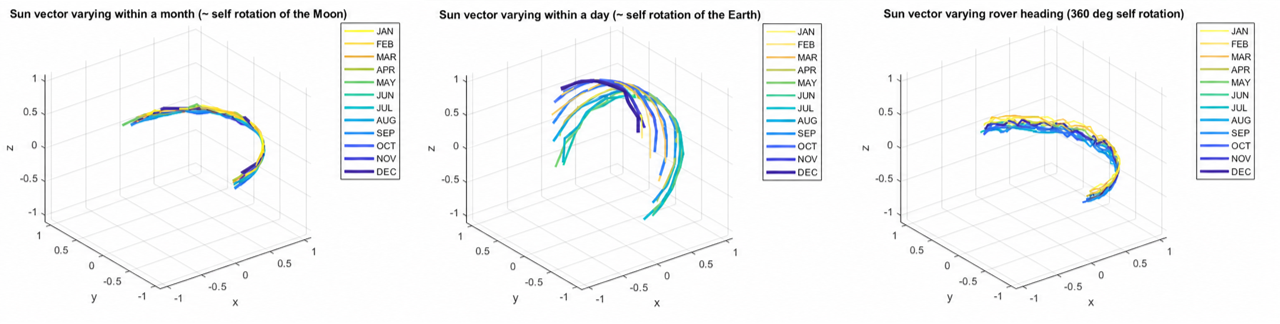
\includegraphics[width=\textwidth]{pics/ephemeris.png}
\caption{Reference vector variation used for the three-axis Sun line-of-sight measurement over month, time of day, and a 360$^\circ$ change in rover heading. Colours indicate monthly trajectories from January to December.}
\label{fig:ephemeris_variation}
\end{figure*}

\subsection{Sun Vector Quaternion Attitude Correction}

The attitude update uses the minimum-rotation quaternion that aligns the predicted Sun vector $\hat S_k^b$ in the body frame from Eq.~\eqref{eq:8} with the measured vector $S_{m,k}^b$ from Eq.~\eqref{eq:9}. Defining their cross and dot products as $c_k$ and $d_k$, respectively, gives
\begin{equation}
\tag{10}\label{eq:10}
\begin{aligned}
c_k
  &=\hat S_k^b\times S_{m,k}^b,\\
d_k
  &=(\hat S_k^b)^\top S_{m,k}^b,\\
\delta q_{\mathrm{FSS},k}
  &=\frac{1}{\sqrt{2(1+d_k)}}
    \begin{bmatrix}1+d_k\\ c_k\end{bmatrix},\\
  &=\begin{bmatrix}\delta q_{w,k}\\ \delta q_{v,k}\end{bmatrix},\\
r_{\mathrm{FSS},k}
  &=2\,\operatorname{sgn}(\delta q_{w,k})\,
    \delta q_{v,k}.
\end{aligned}
\end{equation}
For small attitude errors, the vector part of Eq.~\eqref{eq:10} is equivalent to a rotation vector and is therefore used directly as the three-component ESKF attitude residual. The estimated attitude error is converted to a right-multiplicative correction quaternion and injected into the nominal INS quaternion. A single instantaneous Sun direction cannot observe rotation about the Sun vector itself; the valid attitude observation subspace is therefore the rank-two projector $P_{\perp,k}=I-\hat S_k^b(\hat S_k^b)^\top$. The covariance along the Sun vector axis is inflated, while the remaining degree of freedom is constrained by IMU propagation and inclination referenced to gravity. Antiparallel geometry with $d_k\simeq-1$ and excessive innovations are excluded by the validity gate.

\section{Ackermann Odometry for Four Independently Steered Wheels}

The second aiding channel is wheel odometry from the drive and steering encoders. A conventional bicycle model becomes singular or inaccurate during zero turns and maneuvers with a small radius. The odometry is therefore formulated directly from the geometry of four independently steered wheels.

\subsection{Kinematics of Four Independently Steered Wheels}

As shown in Fig.~\ref{fig:odometry_geometry}, the rover has wheelbase $L$, half-track $d$, and independently steered wheels at the four corners. For instantaneous turning radius $\rho$, the rear steering angles satisfying the Ackermann condition are
\begin{equation}
\tag{11}\label{eq:11}
\delta_{LB}=-\arctan\!\left(\dfrac{L}{\rho-d}\right),\qquad \delta_{RB}=-\arctan\!\left(\dfrac{L}{\rho+d}\right).
\end{equation}
The front axle uses the corresponding equations with opposite sign. The effective rover steering angle is
\begin{equation}
\tag{12}\label{eq:12}
\delta_{\mathrm{rover}}=\tfrac{1}{2}(\delta_{LB}+\delta_{RB}).
\end{equation}

\begin{figure}[t]
\centering
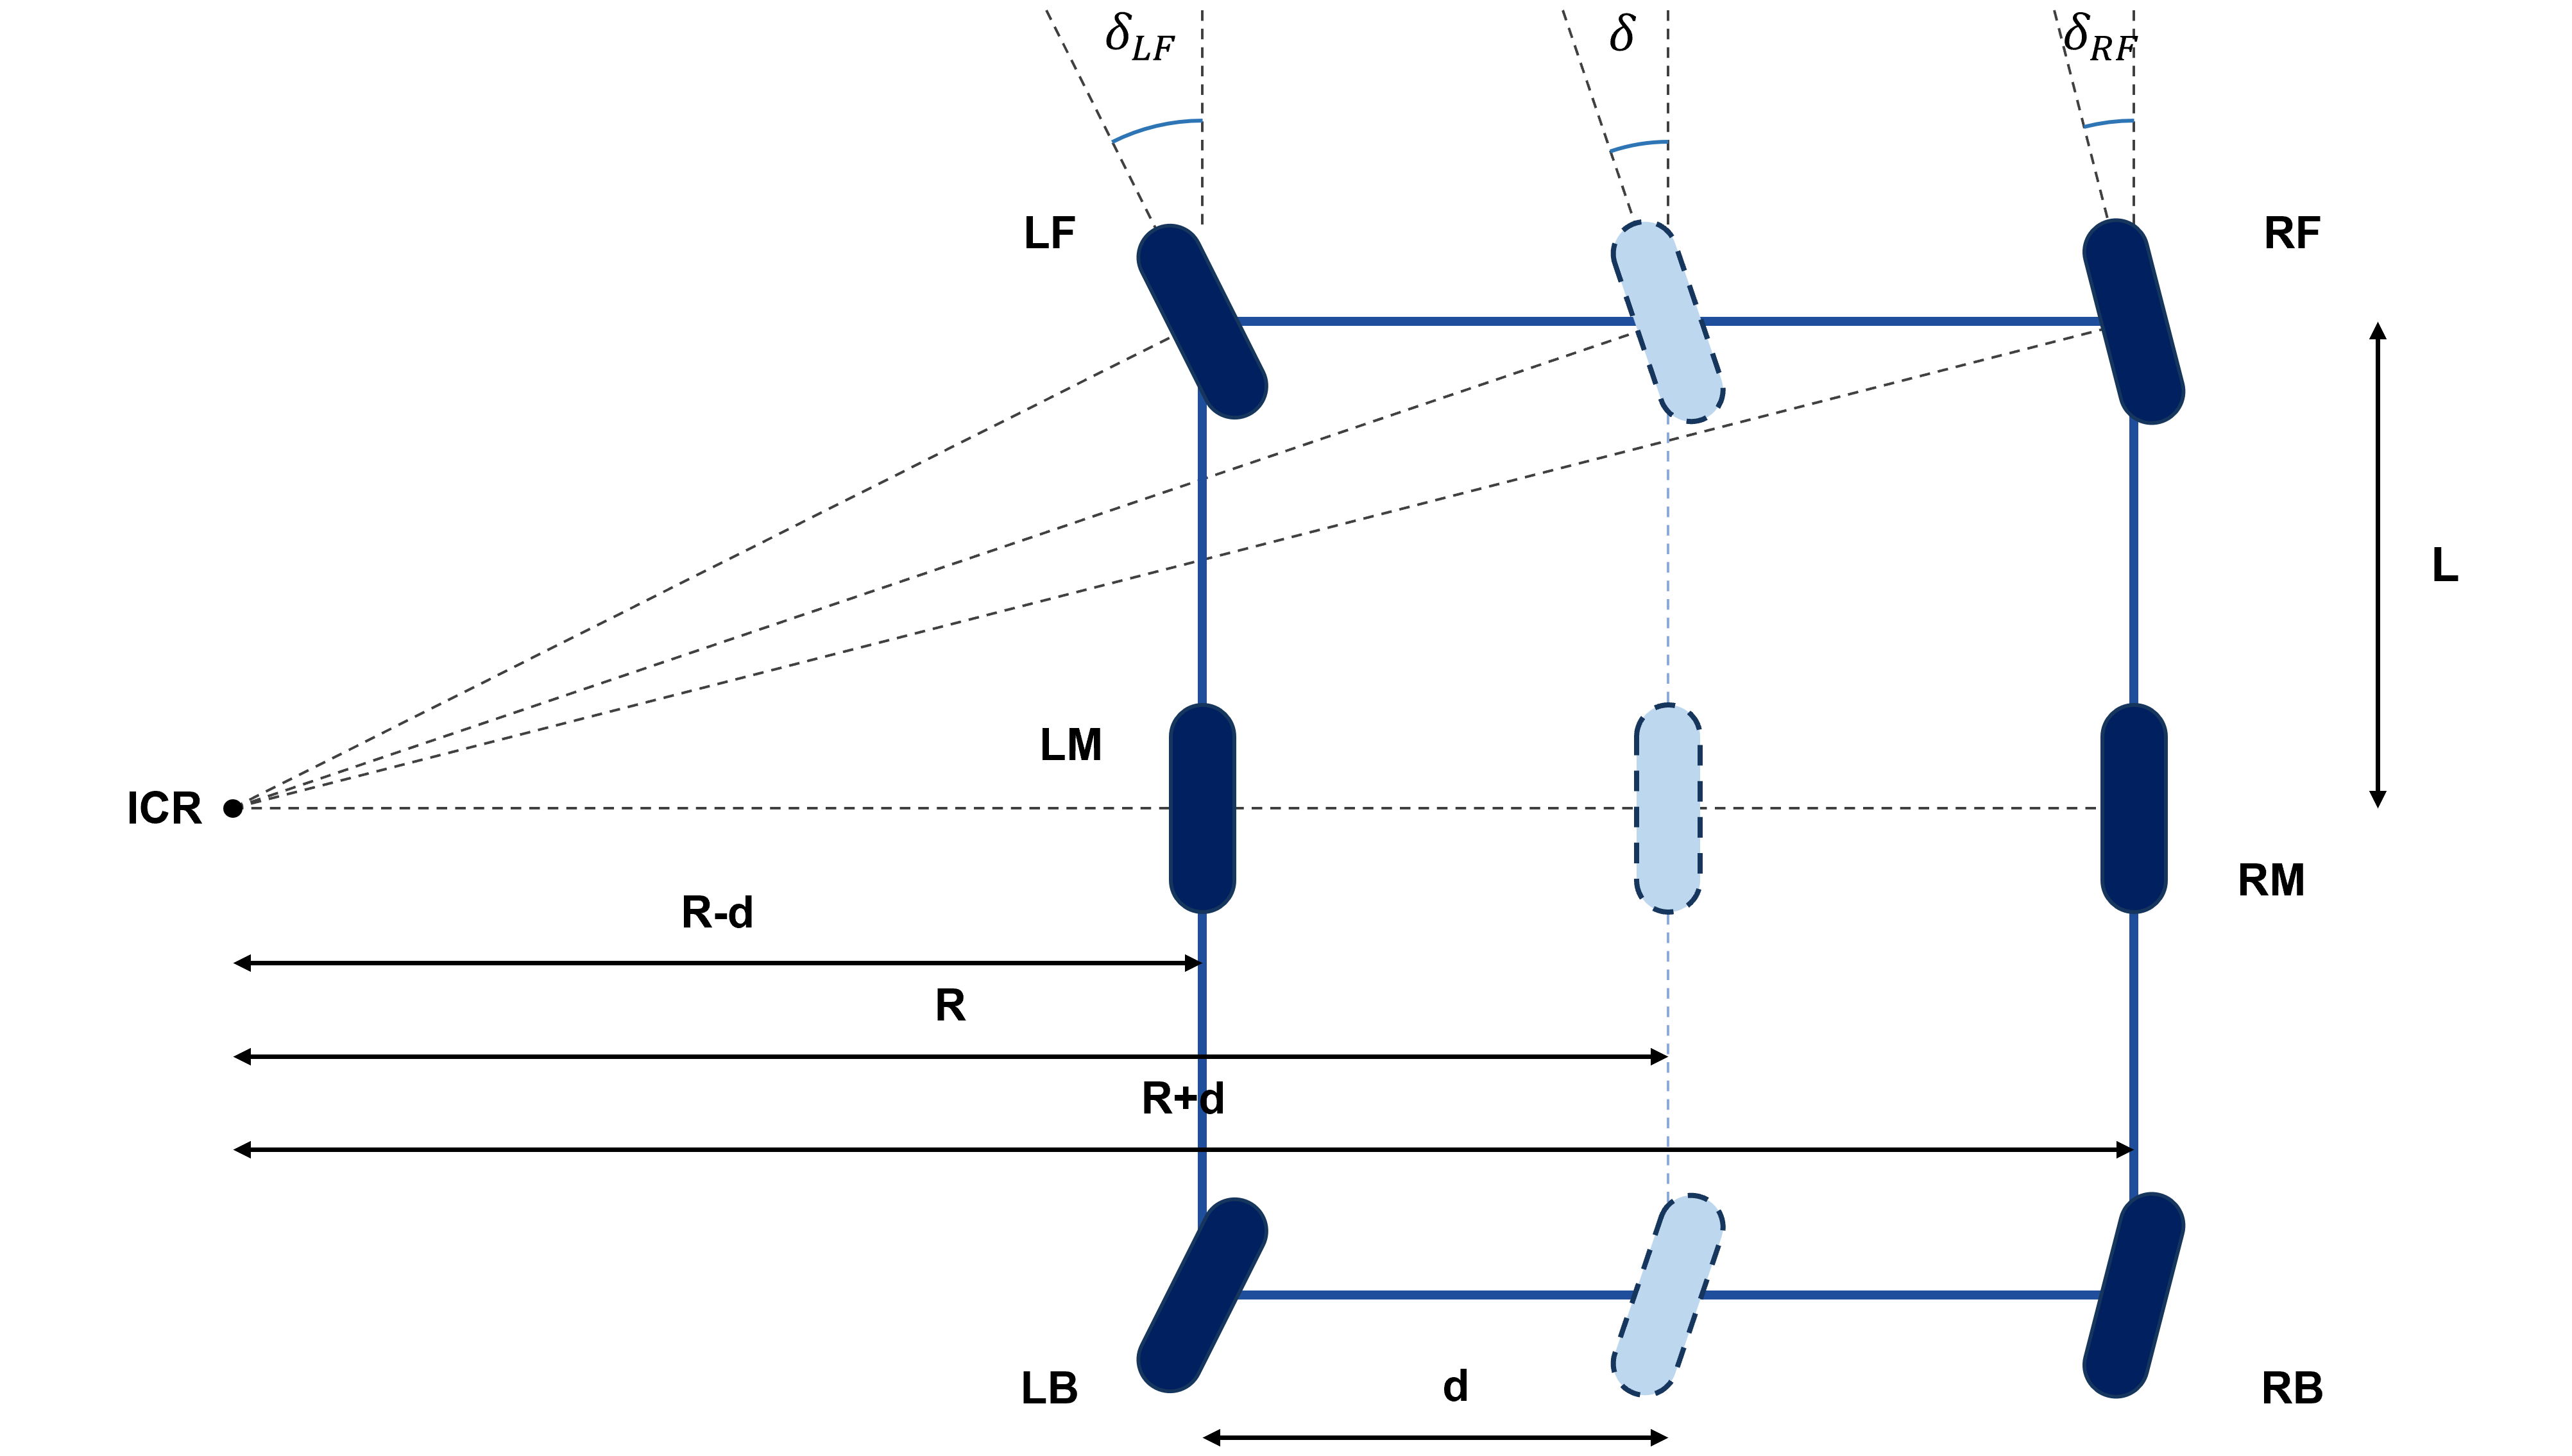
\includegraphics[width=\linewidth]{pics/odometry.png}
\caption{Ackermann geometry and wheel angle definitions for four independently steered wheels about the instantaneous centre of rotation.}
\label{fig:odometry_geometry}
\end{figure}

\subsection{Velocity and Yaw Rate Observations}

The rear drive encoders provide the clearest rolling contact estimates. With wheel radius $r_w$ and rear wheel angular rates $n_{RL}$ and $n_{RR}$,
\begin{equation}
\tag{13}\label{eq:13}
v_{RL}=r_wn_{RL},\qquad v_{RR}=r_wn_{RR}.
\end{equation}
The longitudinal speed, yaw rate, and instantaneous radius are
\begin{equation}
\tag{14}\label{eq:14}
\begin{aligned}
v_{\mathrm{avg}}&=\tfrac12\bigl(v_{RL}+v_{RR}\bigr),\\
\omega_{bz}&=\dfrac{v_{RR}-v_{RL}}{2d},\\
\rho&=\dfrac{v_{\mathrm{avg}}}{\omega_{bz}}.
\end{aligned}
\end{equation}
The odometry pseudo-measurement is
\begin{equation}
\tag{15}\label{eq:15}
y_k^{\mathrm{od}}=\begin{bmatrix}v_{\mathrm{avg}}\\\omega_{bz}\end{bmatrix}+e_{\mathrm{od},k}.
\end{equation}
It is compared with the longitudinal projection of the nominal velocity in the body frame and with the body yaw rate derived from the gyroscope. The covariance is increased with locally estimated slip, reducing the weight of odometry at starts with high slip.

\subsection{Zero Turns and Wheelbase Adjustment}

During a zero turn, all wheels are tangent to a common rotation centre at the body centre. Longitudinal speed is zero while yaw rate is nonzero, so the bicycle model radius becomes singular. The four-wheel model handles the condition directly with $v_{\mathrm{avg}}=0$ and $\omega_{bz}=(v_{RR}-v_{RL})/(2d)\neq0$. During wheelbase adjustment, temporarily nonparallel front and rear steering commands vary the effective kinematic wheelbase. Because the individual steering angles remain explicit, the observation in Eq.~\eqref{eq:15} remains defined throughout both maneuvers.

\section{Error-State Kalman Filter Formulation}

The ESKF is the fusion engine of the proposed system. The nominal state is propagated by nonlinear INS mechanization, while the filter estimates the small error between the nominal and true trajectories. Estimated errors from FSS and wheel odometry updates are injected into the nominal state. A right-multiplicative attitude error convention is used consistently~\cite{lefferts1982kalman,sola2017quaternion,sveinsson2012insgps}.

\subsection{State Decomposition}

The 16-dimensional nominal state consists of position, velocity, unit quaternion attitude, accelerometer bias, and gyro bias:
\begin{equation*}
x=\bigl[(p^\ell)^{\top},(v^\ell)^{\top},(q_b^\ell)^{\top},b_a^{\top},b_g^{\top}\bigr]^{\top}\in\mathbb{R}^{16}.
\end{equation*}
The true state $x_t$ is decomposed with the generalized addition operator $\oplus$:
\begin{equation}
\tag{16}\label{eq:16}
x_t=x\oplus\delta x.
\end{equation}
The error state is reset to zero after each injection into the nominal state.
The component relations are
\begin{equation}
\tag{17}\label{eq:17}
p_t^\ell=p^\ell+\delta p^\ell,\qquad v_t^\ell=v^\ell+\delta v^\ell,\qquad q_{b,t}^\ell=q_b^\ell\otimes\delta q(\delta\theta),
\end{equation}
\begin{equation}
\tag{18}\label{eq:18}
b_{a,t}=b_a+\delta b_a,\qquad b_{g,t}=b_g+\delta b_g.
\end{equation}
The attitude error is the three-component rotation vector $\delta\theta$, and $\delta q(\delta\theta)\simeq[1,\tfrac12\delta\theta^\top]^\top$ for small angles. The 15-dimensional error state is
\begin{equation}
\tag{19}\label{eq:19}
\delta x=\bigl[(\delta p^\ell)^{\top},(\delta v^\ell)^{\top},\delta\theta^{\top},\delta b_a^{\top},\delta b_g^{\top}\bigr]^{\top}\in\mathbb{R}^{15}.
\end{equation}
This formulation avoids directly estimating a correction quaternion under a unit norm constraint.

\subsection{Nominal State Kinematics}

Let $\hat f^b=f_m^b-b_a$ and $\hat\omega_{\ell b}^b=\omega_m^b-b_g$. Over an IMU interval $\Delta t$, the nominal state is propagated as
\begin{equation}
\tag{20}\label{eq:20}
\begin{aligned}
a_k^\ell&=C_b^\ell\hat f_k^b+g^\ell,\\
p_{k+1}^\ell&=p_k^\ell+v_k^\ell\Delta t
  +\tfrac12a_k^\ell\Delta t^2,\\
v_{k+1}^\ell&=v_k^\ell+a_k^\ell\Delta t,\\
\Delta q_k
  &=\operatorname{Exp}_q\!\left(
    \hat\omega_{\ell b,k}^b\Delta t\right),\\
q_{b,k+1}^\ell
  &=\frac{q_{b,k}^\ell\otimes\Delta q_k}
  {\left\lVert q_{b,k}^\ell\otimes\Delta q_k\right\rVert},\\
b_{a,k+1}&=b_{a,k},\\
b_{g,k+1}&=b_{g,k}.
\end{aligned}
\end{equation}
Here, $\operatorname{Exp}_q(\cdot)$ maps a rotation vector to the incremental unit quaternion $\Delta q_k$. IMU white noise and bias random walks are represented through the error state covariance.

\subsection{Error State Kinematics}

Linearization about the nominal trajectory using the right-multiplicative error gives
\begin{equation}
\tag{21}\label{eq:21}
\begin{aligned}
\delta\dot p^\ell&=\delta v^\ell,\\
\delta\dot v^\ell
  &=-C_b^\ell[\hat f^b]_\times\delta\theta-C_b^\ell\delta b_a\\
  &\quad{}-C_b^\ell n_a,\\
\delta\dot\theta
  &=-[\hat\omega_{\ell b}^b]_\times\delta\theta-\delta b_g-n_g,\\
\delta\dot b_a&=n_{wa},\\
\delta\dot b_g&=n_{wg}.
\end{aligned}
\end{equation}
Here, $[\cdot]_\times$ is the skew-symmetric cross product matrix; $n_a$ and $n_g$ are accelerometer and gyro white noise; and $n_{wa}$ and $n_{wg}$ drive the bias random walks.

\subsection{Covariance Propagation and Noise Discretization}

The continuous and discrete error dynamics are
\begin{equation}
\tag{22}\label{eq:22}
\begin{aligned}\delta\dot x&=F_c\delta x+G_cw,\\\delta x_{k+1}&=\Phi_k\delta x_k+w_{d,k},\\\Phi_k&=\exp(F_c\Delta t).\end{aligned}
\end{equation}
Here, $w=[n_a^\top,n_g^\top,n_{wa}^\top,n_{wg}^\top]^\top$ is the continuous-time noise vector, and $\Phi(\tau)=\exp(F_c\tau)$ is the state transition matrix over an interval $\tau$.
For the local Cartesian model over short ranges,
\begin{equation}
\tag{23a}\label{eq:23a}
A_f\equiv[\hat f^b]_\times,
\qquad
A_\omega\equiv[\hat\omega_{\ell b}^b]_\times.
\end{equation}
\begin{equation}
\tag{23b}\label{eq:23b}
F_c=
\begin{bmatrix}
0&I&0&0&0\\
0&0&-C_b^\ell A_f&-C_b^\ell&0\\
0&0&-A_\omega&0&-I\\
0&0&0&0&0\\
0&0&0&0&0
\end{bmatrix}.
\end{equation}
\begin{equation}
\tag{23c}\label{eq:23c}
G_c=
\begin{bmatrix}
0&0&0&0\\
-C_b^\ell&0&0&0\\
0&-I&0&0\\
0&0&I&0\\
0&0&0&I
\end{bmatrix}.
\end{equation}
With continuous-time noise power spectral density $Q_c$,
\begin{equation}
\tag{24}\label{eq:24}
\begin{aligned}Q_{d,k}&=\int_0^{\Delta t}\Phi(\tau)G_cQ_cG_c^\top\Phi^\top(\tau)\,d\tau\\&\simeq G_cQ_cG_c^\top\Delta t,\\P_{k+1}^-&=\Phi_kP_k^+\Phi_k^\top+Q_{d,k}.\end{aligned}
\end{equation}
For small $\Delta t$, $\Phi_k\simeq I+F_c\Delta t$. No additional $\Delta t$ is applied after $Q_{d,k}$ has been discretized.

\subsection{Measurement Update}

FSS and wheel odometry measurements are processed asynchronously through nonlinear functions $h_j(x)$:
\begin{equation}
\tag{25}\label{eq:25}
\begin{aligned}r_k&=z_k-h_j(x_k^-),\\H_k&=\left.\frac{\partial h_j(x_k^-\oplus\delta x)}{\partial\delta x}\right|_{\delta x=0}.\end{aligned}
\end{equation}
The FSS update uses the attitude residual $r_{\mathrm{FSS},k}$ formed from the vector part of the correction quaternion in Eq.~\eqref{eq:10}. With the right-multiplicative error convention and the cross product order in Eq.~\eqref{eq:10}, the attitude block of the measurement Jacobian is $H_{\mathrm{FSS},\theta}=-P_{\perp,k}$. This projection prevents correction about the unobservable Sun axis. For a Jacobian $H_x$ with respect to the full nominal state, $H_k=H_xX_\delta$, where
\begin{equation}
\tag{26}\label{eq:26}
\begin{aligned}X_\delta&=\operatorname{blkdiag}(I_6,Q_{\delta\theta},I_6),\\Q_{\delta\theta}&=\frac12\begin{bmatrix}-q_v^\top\\q_wI+[q_v]_\times\end{bmatrix},\\q&=[q_w,\ q_v^\top]^\top.\end{aligned}
\end{equation}
The innovation covariance and Kalman gain are
\begin{equation}
\tag{27}\label{eq:27}
\begin{aligned}S_k&=H_kP_k^-H_k^\top+R_k,\\K_k&=P_k^-H_k^\top S_k^{-1}.\end{aligned}
\end{equation}
The error state mean and covariance are updated in Joseph form:
\begin{equation}
\tag{28}\label{eq:28}
\begin{aligned}
\delta\hat x_k&=K_kr_k,\\
P_k^+
  &=(I-K_kH_k)P_k^-(I-K_kH_k)^\top\\
  &\quad{}+K_kR_kK_k^\top.
\end{aligned}
\end{equation}
Joseph form helps preserve covariance symmetry and positive semidefiniteness under finite-precision arithmetic.

\subsection{Error Injection and Reset}

After each measurement update, the estimated error is injected into the nominal state. With the right-multiplicative convention,
\begin{equation}
\tag{29a}\label{eq:29a}
\begin{aligned}
p^\ell&\leftarrow p^\ell+\delta\hat p^\ell,
&v^\ell&\leftarrow v^\ell+\delta\hat v^\ell,\\
q_b^\ell&\leftarrow
  \frac{q_b^\ell\otimes\delta q(\delta\hat\theta)}
  {\left\lVert q_b^\ell\otimes\delta q(\delta\hat\theta)\right\rVert},\\
b_a&\leftarrow b_a+\delta\hat b_a,
&b_g&\leftarrow b_g+\delta\hat b_g.
\end{aligned}
\end{equation}
\begin{equation}
\tag{29b}\label{eq:29b}
\begin{aligned}
G_{\mathrm{reset}}
  &=\operatorname{blkdiag}\!\left(
    I_6,I-\tfrac12[\delta\hat\theta]_\times,I_6\right),\\
P&\leftarrow G_{\mathrm{reset}}P^+G_{\mathrm{reset}}^\top,
&\delta\hat x&\leftarrow0.
\end{aligned}
\end{equation}
The corrected nominal state becomes the next linearization point. The quaternion is normalized after each injection, and the bias ordering $[b_a,b_g]$ is kept consistent in the state and covariance~\cite{sola2017quaternion}.

\section{Simulation}

The lunar rover environment is implemented using Microsoft AirSim and Unreal Engine. It includes constant lunar gravity, synthetic terrain, the kinematics of four independently steered wheels, and interaction between the wheels and terrain. IMU, FSS, and encoder sampling, noise, bias, and time synchronization are defined, and the simulated sensor data are supplied to the ESKF. Figure~\ref{fig:lunar_simulation_environment} shows the terrain and rover driving environment.

The simulation uses the lunar gravity model and takes the rover pose reported by Unreal Engine as ground truth. INS propagation driven by the IMU, the FSS measurement update, and the wheel odometry update operate at 200~Hz, 5~Hz, and 20~Hz, respectively. Four manoeuvre types are exercised: straight driving, turning, slope traversal, and a composite route, with wheel slip intervals included in the route. The simulated IMU and FSS noise and bias are constructed from the sensor class specifications in Table~\ref{tab:sensors}. The initial covariance $P_0$, process noise covariance $Q$, and measurement noise covariance $R$ are diagonal matrices derived from the sensor specifications. After software simulation, the same sensor input and update paths are executed on the physical NAVCOM through PILS/HILS to verify coordinate transformations, execution cadence, and data flow in real time.

\begin{figure}[!t]
\centering
\begin{subfigure}[t]{0.98\linewidth}
  \centering
  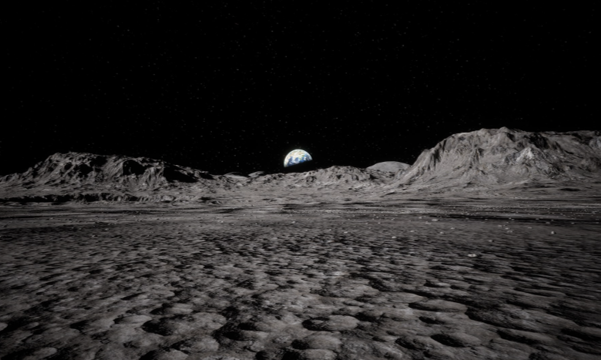
\includegraphics[width=\linewidth]{pics/moon.png}
  \caption{Lunar terrain scene}
\end{subfigure}
\par\medskip
\begin{subfigure}[t]{0.98\linewidth}
  \centering
  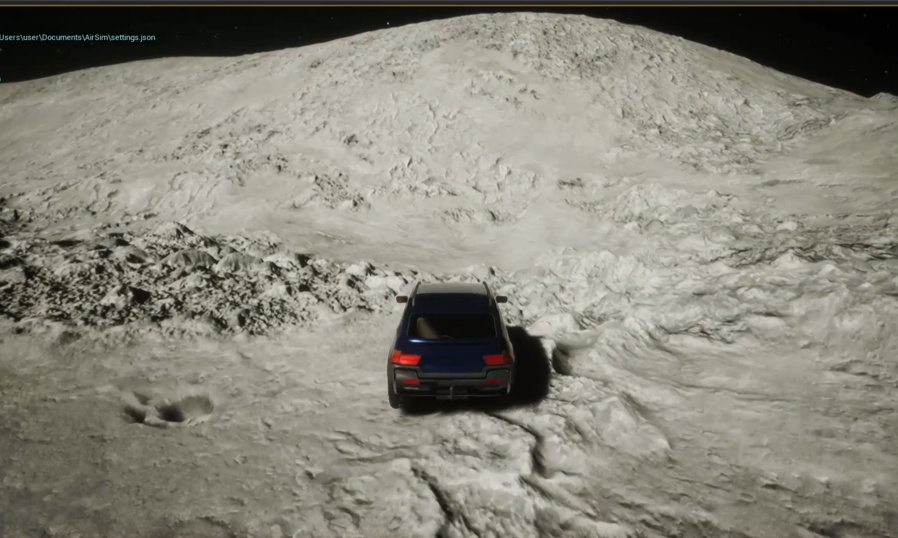
\includegraphics[width=\linewidth]{pics/sim_moon_car_crop.png}
  \caption{Rover driving simulation}
\end{subfigure}
\par\medskip
\begin{subfigure}[t]{0.98\linewidth}
  \centering
  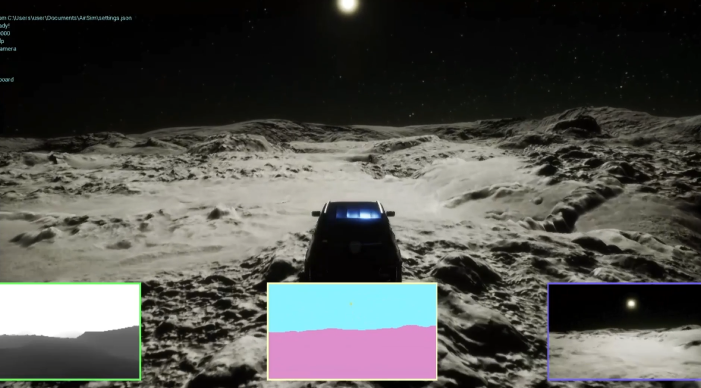
\includegraphics[width=\linewidth]{pics/sim_moon_car2.png}
  \caption{Rover driving and simulated sensor views}
\end{subfigure}
\caption{Unreal Engine/AirSim lunar terrain and rover driving simulation environment.}
\label{fig:lunar_simulation_environment}
\end{figure}

In the FSS simulation, the reference Sun vector is computed from rover position and time, transformed through MCI to MCMF and then through the fixed local frame at the landing site, and expressed in the sensor frame. Angular noise and bias representative of the FSS are added.

\subsection{Simulation Results}

The reported simulation evaluates the tracking performance of the integrated INS + wheel odometry + FSS configuration. Wheel odometry velocity observations and the FSS Sun vector quaternion correction are processed asynchronously while the nominal INS state is propagated. Repeated executions of the identically defined scenario were used to check implementation repeatability, and the paper presents one representative time history. Ensemble statistics are outside the scope of this study; therefore, the results are not interpreted as a Monte Carlo performance assessment.

Figure~\ref{fig:simulation_navigation_results} presents the attitude, velocity, and position tracking results for the integrated configuration. The ``INS Result'' label embedded in the plots denotes the nominal INS navigation state after ESKF measurement updates and error injection.

The estimated roll, pitch, and yaw generally follow the reference attitude variations. The correction quaternion formed from the measured three-axis Sun vector and the reference vector derived from ephemeris data is supplied to the ESKF attitude update, thereby limiting the accumulation of inertial attitude error over time. The wheel odometry observation constrains planar speed and maintains tracking of the $x$ and $y$ velocity components. Short transient differences appear in the vertical component during abrupt terrain changes, after which the estimate returns toward the reference. The horizontal position components also closely follow the reference trajectory, whereas the vertical position exhibits comparatively larger transient errors because it depends on terrain height variation and integrated vertical acceleration.

\begin{figure}[H]
\centering
\begin{subfigure}[t]{0.98\linewidth}
  \centering
  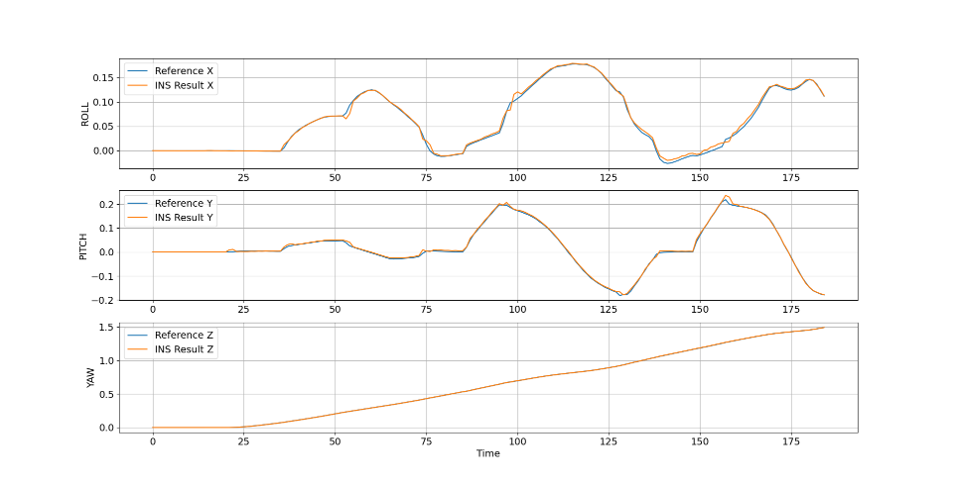
\includegraphics[width=\linewidth]{pics/atti.png}
  \caption{Roll, pitch, and yaw attitude components}
\end{subfigure}
\par\medskip
\begin{subfigure}[t]{0.98\linewidth}
  \centering
  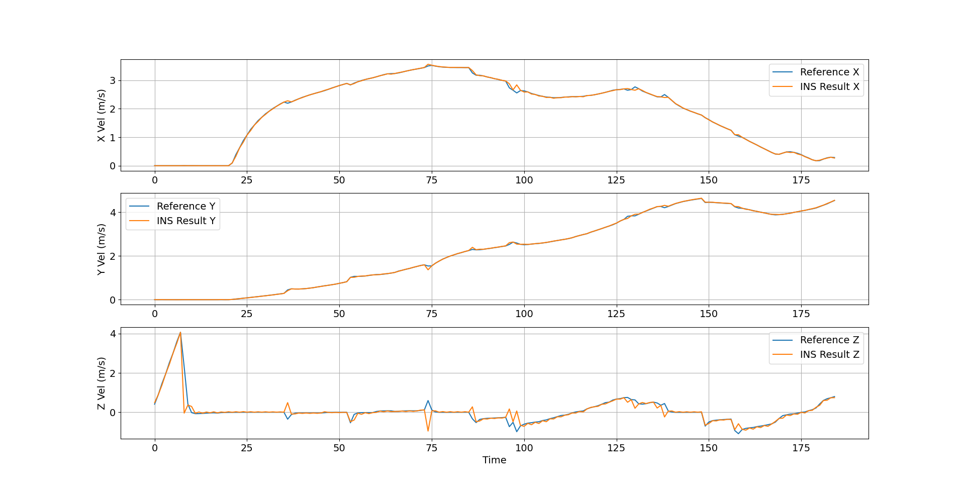
\includegraphics[width=\linewidth]{pics/vel.png}
  \caption{Three-axis velocity components}
\end{subfigure}
\par\medskip
\begin{subfigure}[t]{0.98\linewidth}
  \centering
  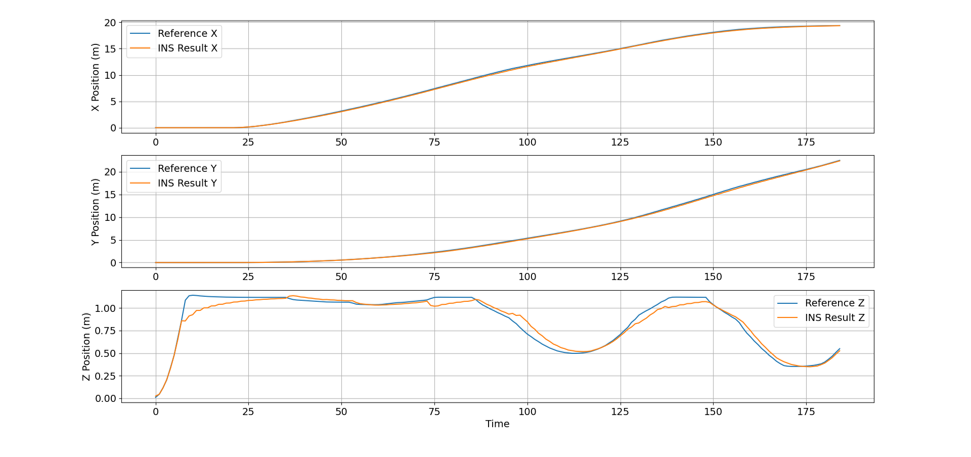
\includegraphics[width=\linewidth]{pics/position.png}
  \caption{Three-axis position components}
\end{subfigure}
\caption{Reference and corrected nominal INS attitude, velocity, and position histories for the INS + wheel odometry + FSS simulation. ``INS Result'' in the embedded plot legends denotes the navigation state after ESKF measurement updates and error injection.}
\label{fig:simulation_navigation_results}
\end{figure}

\section{Hardware Tests}

\subsection{Hardware Configuration}

A full-scale rover with four independently steered wheels is used to evaluate real-time implementation and practical applicability. The rover carries a Jetson Orin Nano/STM32F7 NAVCOM, an IMU, four wheel encoders, steering angle sensors, and three FSS units, as shown in Fig.~\ref{fig:hw_architecture}. The STM32F7 collects encoder, steering, and low-level drivetrain data; the Jetson performs time synchronization, four-wheel odometry, and real-time ESKF navigation. The FSS channels were not activated in the indoor hardware tests because representative solar illumination could not be reproduced.

\begin{figure*}[!t]
\centering
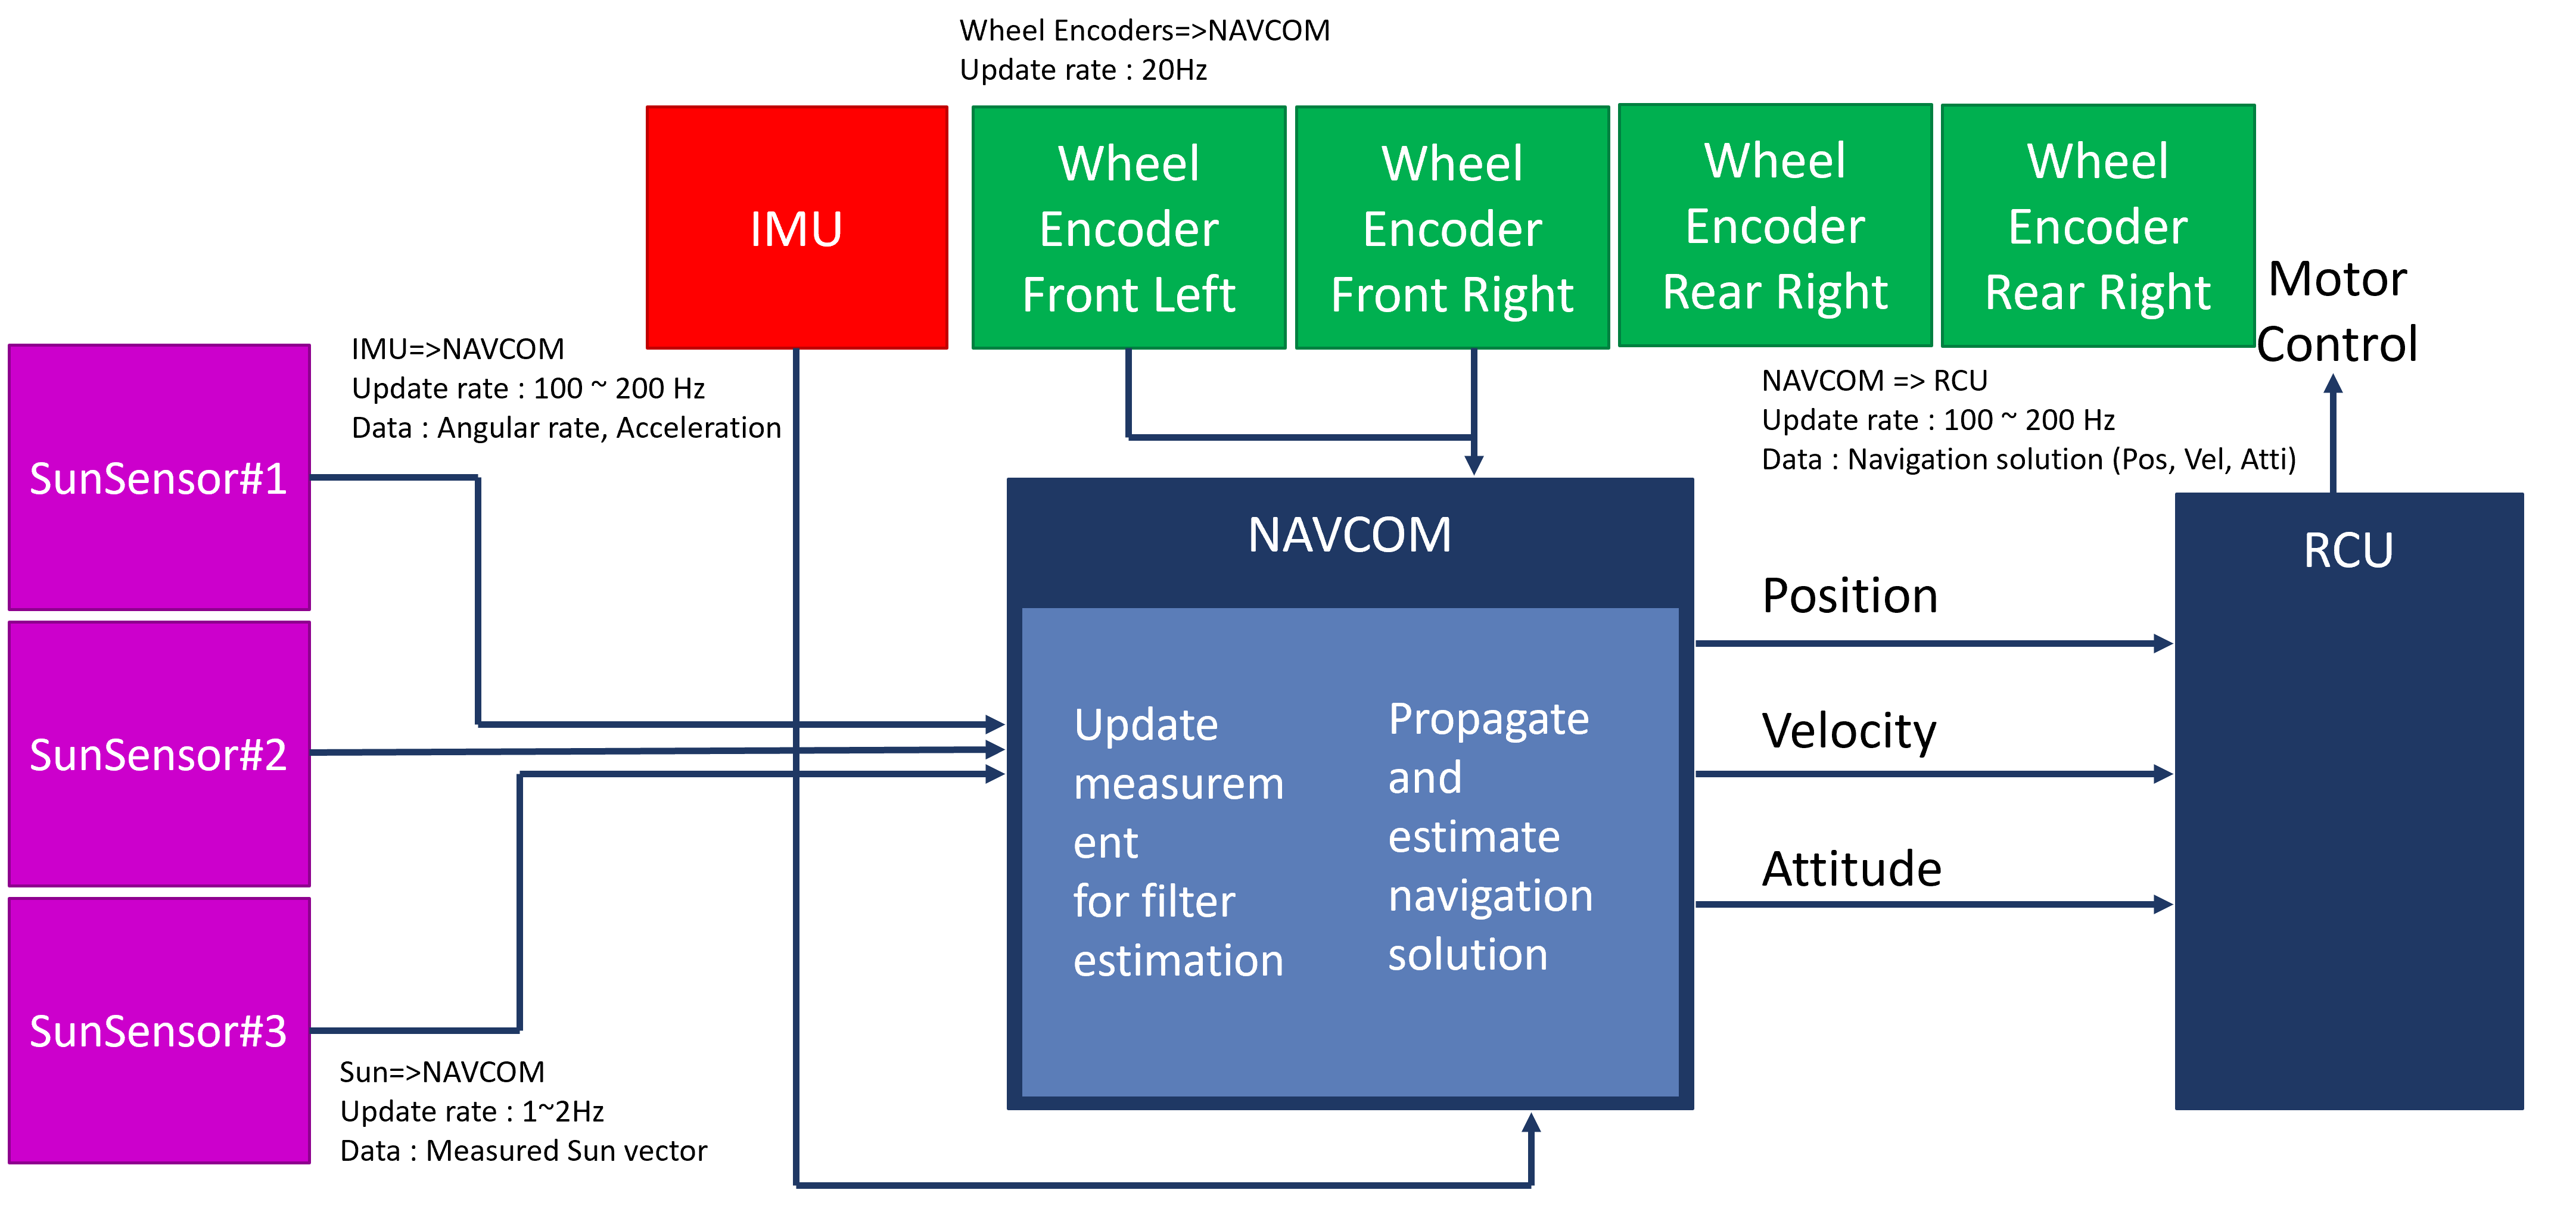
\includegraphics[width=\textwidth]{pics/hw_architecture.png}
\caption{Navigation hardware (NAVCOM) architecture of the full-scale rover.}
\label{fig:hw_architecture}
\end{figure*}

\subsection{Test Environment}
\label{sec:hardware_test_environment}

Two complementary ground-test environments were constructed. First, an artificial lunar regolith bed containing prepared pits and uneven regions was used to examine wheel sinkage, traction loss, and slip-induced odometry disturbances. Figure~\ref{fig:regolith_pit} shows representative pits and disturbed surface regions introduced along the driving path. Second, a lunar analogue terrain constructed from Isopink rigid foam panels was used to reproduce larger-scale lunar surface geometry, including slopes and local relief. Rover driving experiments were conducted in both environments to exercise the navigation system under wheel slip and terrain-induced contact disturbances.

\begin{figure}[!t]
\centering
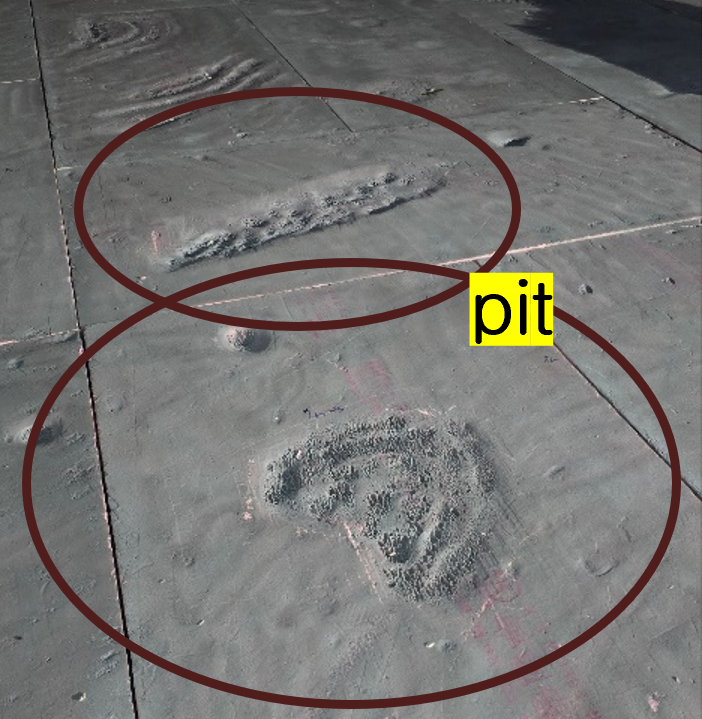
\includegraphics[width=\linewidth]{pics/pit.png}
\caption{Artificial lunar regolith test surface with prepared pits and disturbed regions used to induce wheel slip and contact disturbances.}
\label{fig:regolith_pit}
\end{figure}

To emulate reduced lunar gravity during ground tests, the rover was connected to a gravity compensation device based on helium buoyancy. The device supported approximately $5/6$ of the rover weight upward, reducing the effective normal load at the contacts between the wheels and terrain to about $1/6$ of its terrestrial value. This arrangement enabled hardware evaluation of wheel sinkage and slip under a normal load condition representative of lunar gravity. The rover inertia remained unchanged; therefore, the apparatus reproduced loading determined by gravity rather than the complete six-degree-of-freedom lunar dynamics.

\subsection{Abnormal State Detection and Filter Reinitialization}
\label{sec:recovery_reinitialization}

During runs on the artificial lunar regolith, pits, obstacles, and transient impacts between the wheels and terrain can abruptly change wheel contact and drive the velocity observations derived from encoder data and the filter tracking states outside their normal operating ranges. The hardware implementation therefore includes a supervisory layer that continuously monitors the wheel odometry velocity and the corresponding filter states. When a predefined threshold is exceeded, the interval is classified as abnormal and the contaminated wheel odometry update is temporarily rejected. The mean of the error state is returned to zero, while the covariance and internal filter information are restored to their initial operating conditions. Wheel odometry updates resume after the measurements and estimated states return to the normal range.

Figure~\ref{fig:filter_reinitialization} shows the interval in which pit and wheel contact disturbances drive the estimated speed outside the normal range and the subsequent return to stable tracking after reinitialization. The complete time history and the enlarged interval are shown together to compare the estimated velocity before and after recovery.

\begin{figure}[H]
\centering
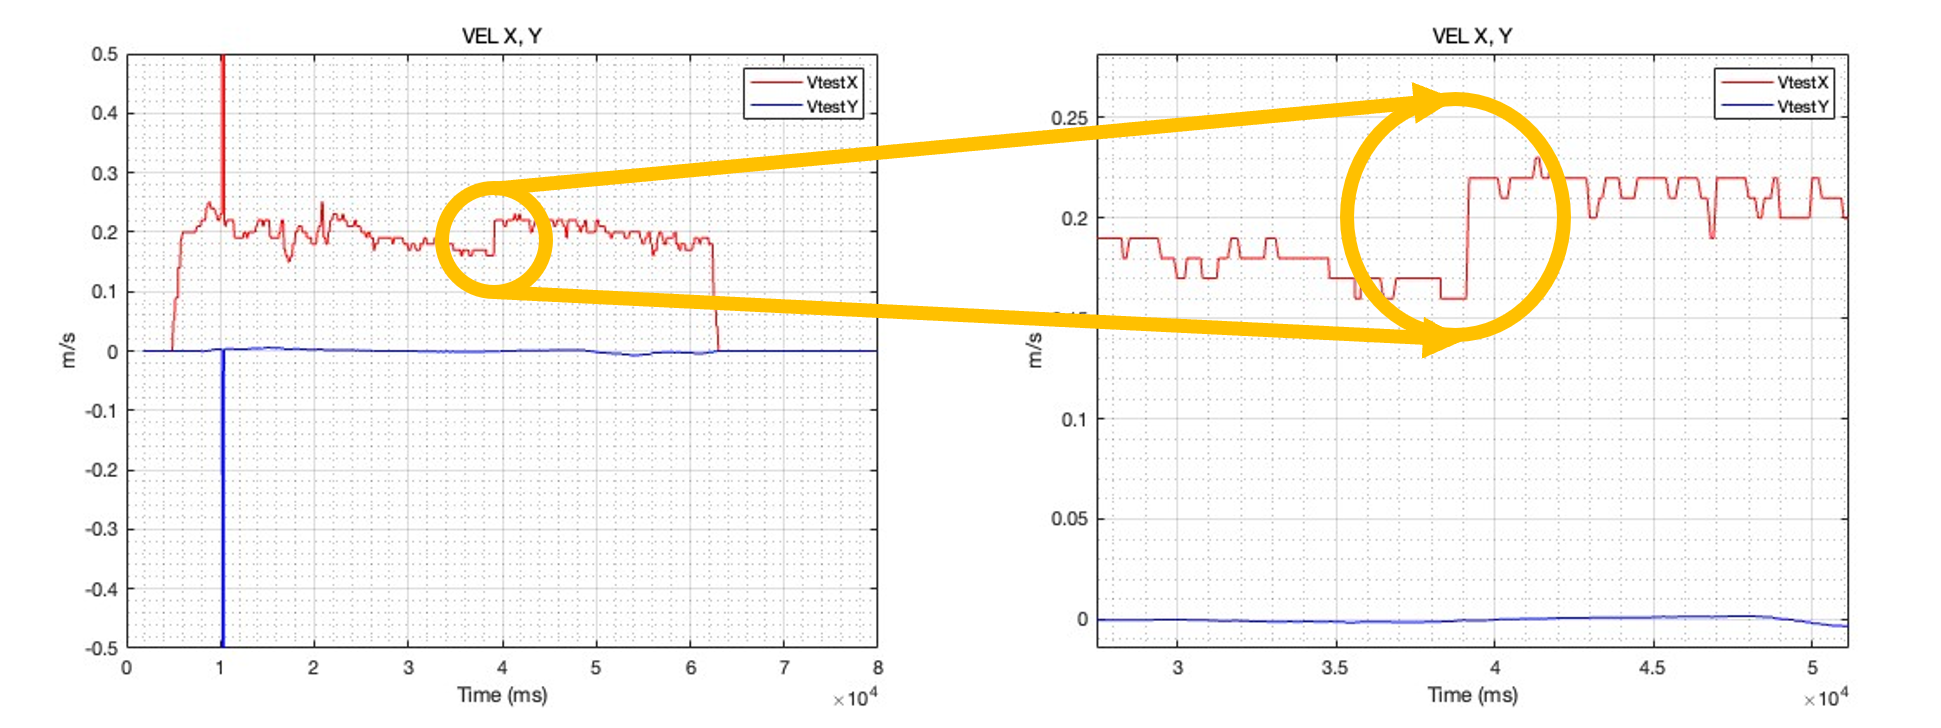
\includegraphics[width=\linewidth]{pics/filter_reinit.png}
\caption{Detection and filter reinitialization when pit and wheel contact disturbances drive the velocity estimate outside its normal range. Insets show the estimate before and after recovery.}
\label{fig:filter_reinitialization}
\end{figure}

This filter reinitialization is a procedure for responding to faults during hardware tests and is distinct from the routine error injection and zero reset performed after each measurement update in Eqs.~\eqref{eq:29a} and~\eqref{eq:29b}. Its purpose is to prevent a gross disturbance from propagating into subsequent position and attitude estimates; the classification of failure modes, effects, and mitigation actions at the system level follows FMECA practice~\cite{borgovini1993fmeca}.

\FloatBarrier

\subsection{Hardware Experimental Results}

The filter reinitialization procedure described in Sec.~\ref{sec:recovery_reinitialization} was activated during the hardware runs. The experiment verified that velocity disturbances generated while traversing pits and obstacles were detected as abnormal, the contaminated wheel odometry updates were rejected, and the filter returned to stable tracking after reinitialization.

Additional time histories from a representative driving run are shown in Figs.~\ref{fig:hardware_drive_velocity} and~\ref{fig:hardware_drive_position}. The longitudinal and lateral plots compare the corrected, provided, INS, and filtered velocity channels; the longitudinal panel also includes the rear-wheel speed signals used by the odometry channel. The planar trajectory shows the position accumulated over the same type of hardware drive. The test logger retains the labels North and East, which correspond in these local experiments to the initially aligned $x_\ell$ and $y_\ell$ axes defined in Sec.~2.2 rather than to a globally referenced lunar NED frame.

\begin{figure}[!t]
\centering
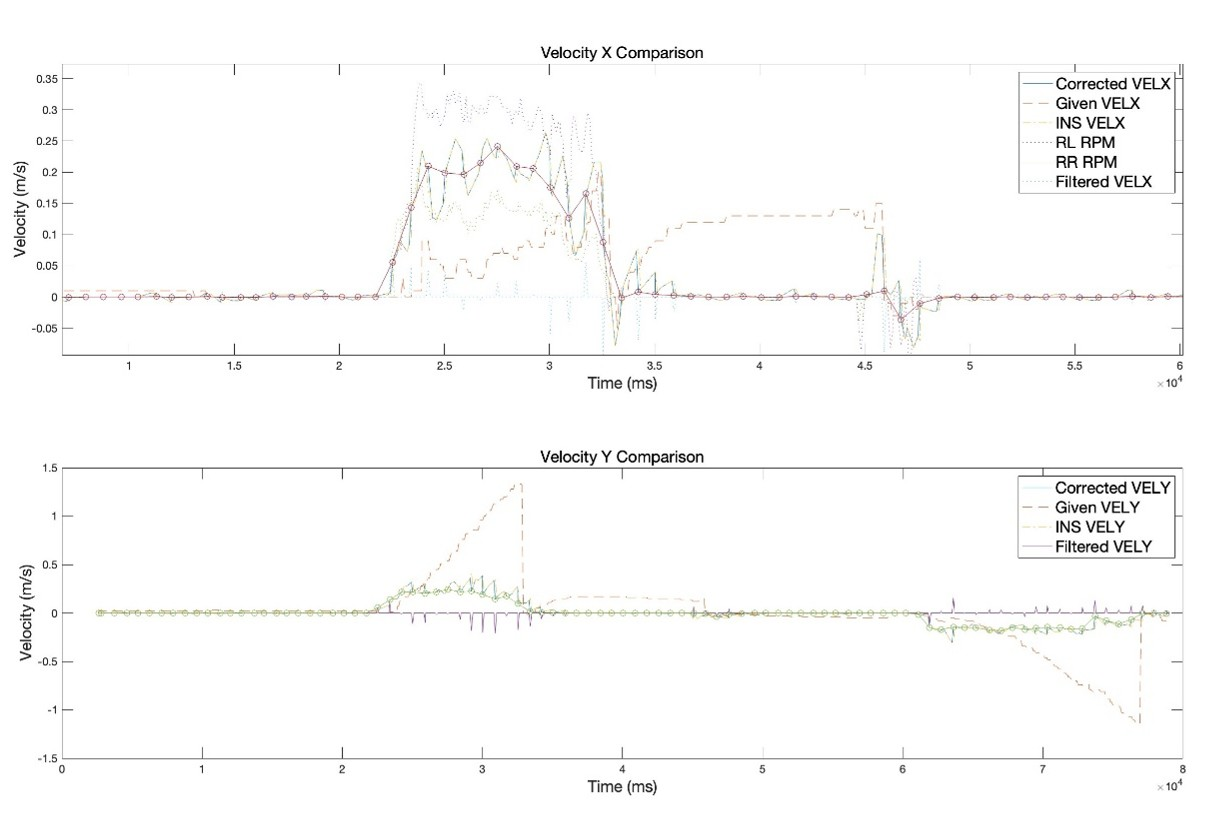
\includegraphics[width=\columnwidth]{pics/drive_result.jpg}
\caption{Longitudinal and lateral velocity histories from a representative hardware driving experiment. Rear-wheel speed signals are also shown in the longitudinal panel.}
\label{fig:hardware_drive_velocity}
\end{figure}

\begin{figure}[!t]
\centering
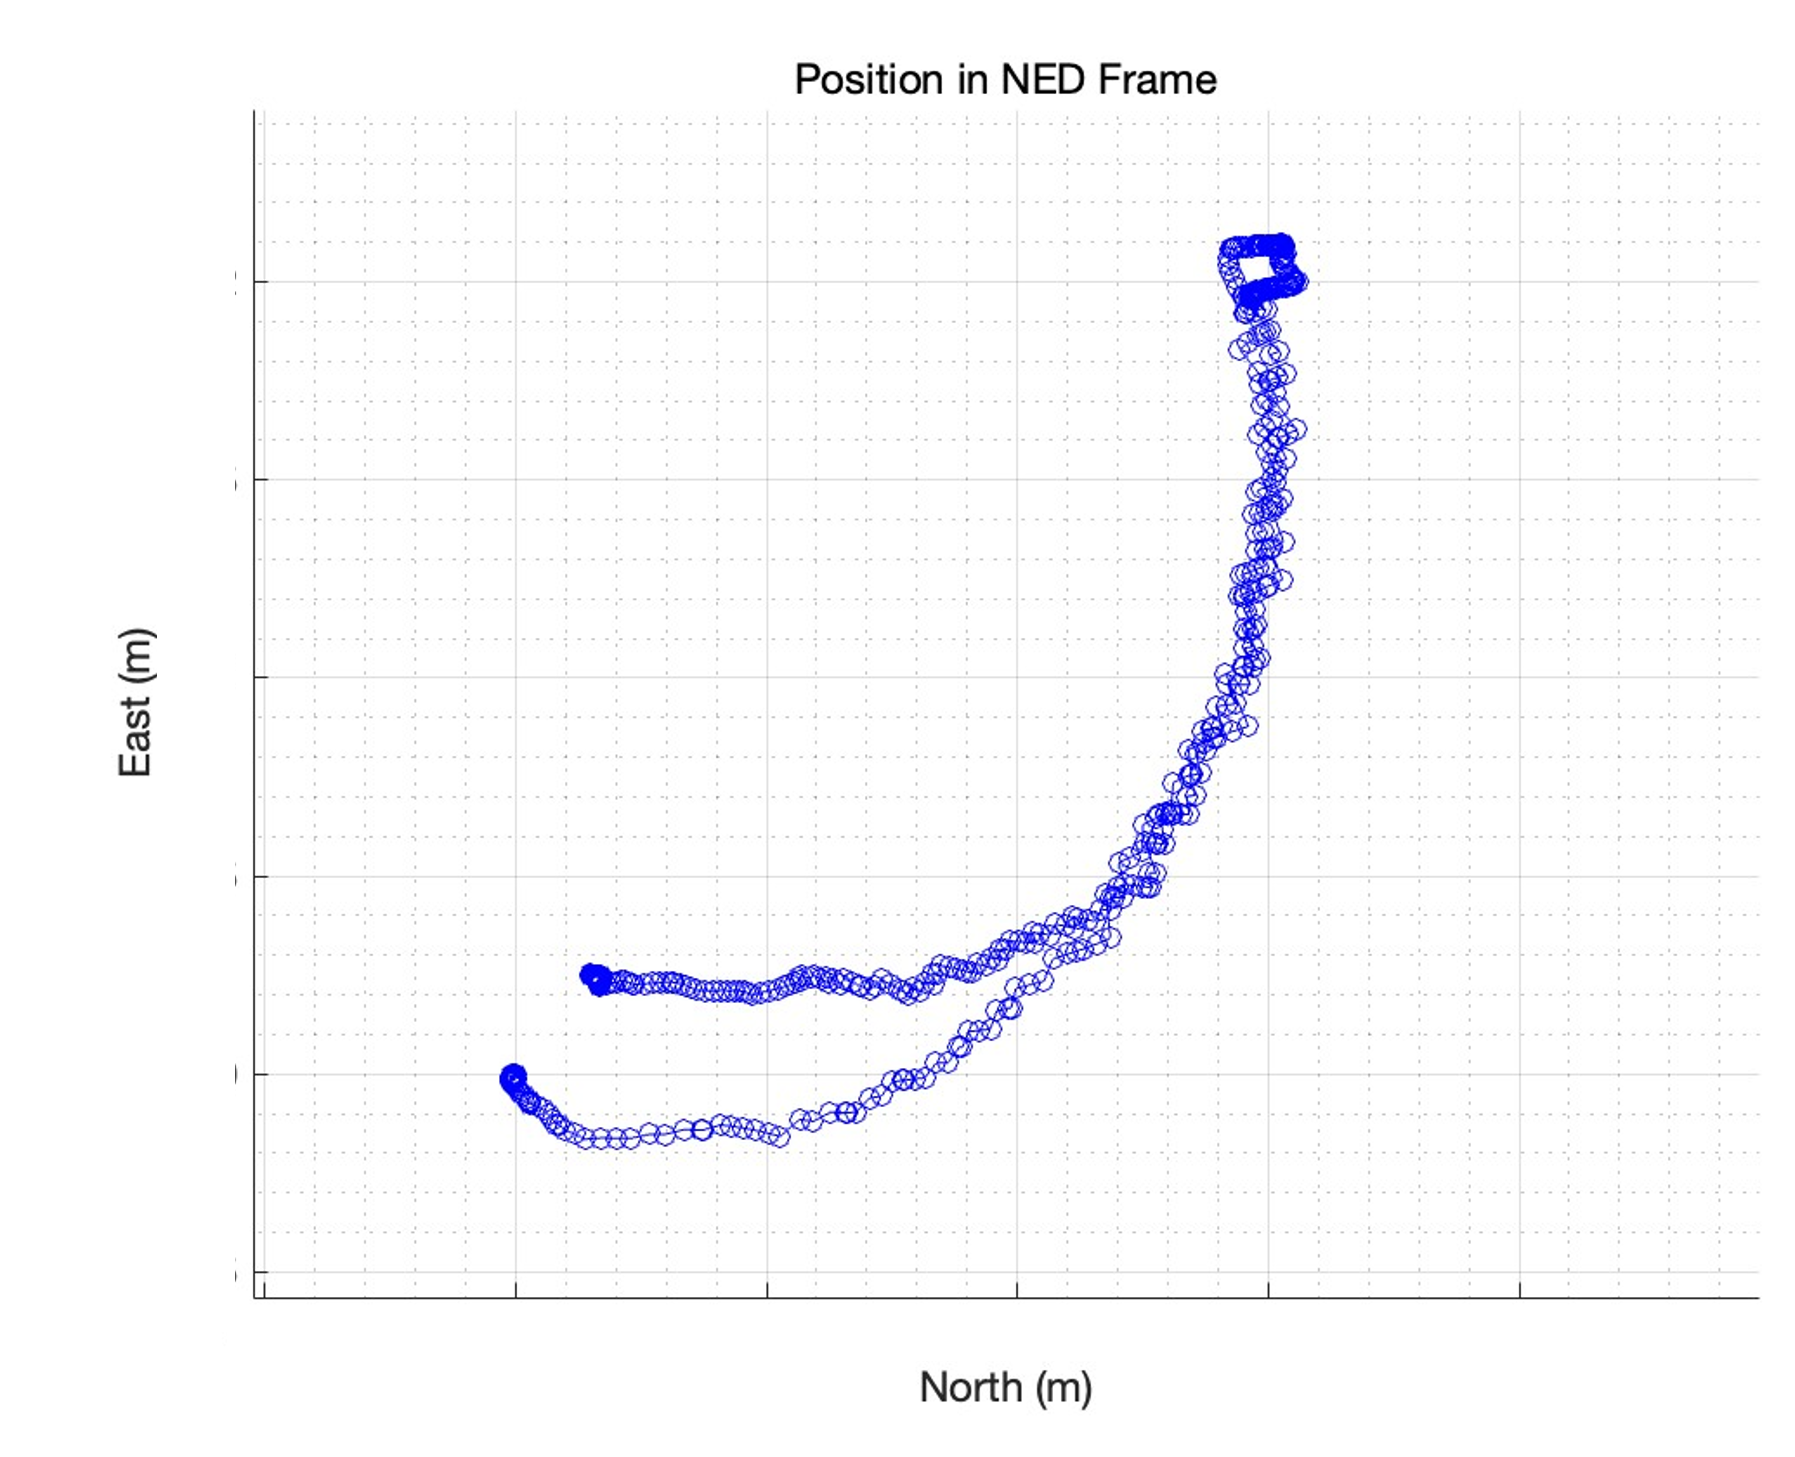
\includegraphics[width=\columnwidth]{pics/result2.png}
\caption{Planar position trajectory from a representative hardware driving experiment. The logger's North and East labels correspond to the locally initialized $x_\ell$ and $y_\ell$ axes used in this study.}
\label{fig:hardware_drive_position}
\end{figure}

Position estimates are compared with laser range measurements, and heading estimates are compared with manually surveyed values in Tables~\ref{tab:position_results} and~\ref{tab:heading_results}. To summarize trials with different terminal displacements, the normalized terminal horizontal position error for run $i$ is defined as $100\lVert p_{\mathrm{est},xy,i}^{\ell}-p_{\mathrm{meas},xy,i}^{\ell}\rVert_2/\lVert p_{\mathrm{meas},xy,i}^{\ell}\rVert_2$. The arithmetic mean over the four position trials is 4.55\% (mean Euclidean terminal error: 0.199~m; maximum normalized error: 8.50\%). The mean absolute heading error over the three heading trials is 0.257$^\circ$ (maximum: 0.57$^\circ$). These values are descriptive statistics of the endpoint comparisons in the tables rather than full-trajectory error measures.

\begin{table}[!t]
\centering
\caption{Position estimation results from the indoor rover experiments. All values are in metres.}
\label{tab:position_results}
\scriptsize
\setlength{\tabcolsep}{2.6pt}
\renewcommand{\arraystretch}{1.10}
\begin{tabularx}{\columnwidth}{l*{4}{>{\centering\arraybackslash}X}}
\toprule
\textbf{Case} & \shortstack{\textbf{Measured}\\\boldmath{$x$}} & \shortstack{\textbf{Measured}\\\boldmath{$y$}} & \shortstack{\textbf{Estimated}\\\boldmath{$x$}} & \shortstack{\textbf{Estimated}\\\boldmath{$y$}} \\
\midrule
MD\#1 & 12.92 &  0.10 & 13.02 &  0.10 \\
MD\#2 &  3.09 & -0.86 &  3.04 & -0.83 \\
MD\#3 &  5.07 &  0.50 &  5.43 &  0.53 \\
AD\#1 &  3.05 & -1.16 &  3.30 & -1.28 \\
\bottomrule
\end{tabularx}
\end{table}

\begin{table}[!t]
\centering
\caption{Heading estimation results from the indoor rover experiments. Heading values are in degrees.}
\label{tab:heading_results}
\scriptsize
\setlength{\tabcolsep}{3.2pt}
\renewcommand{\arraystretch}{1.10}
\begin{tabularx}{\columnwidth}{lcc>{\centering\arraybackslash}X}
\toprule
\textbf{Case} & \shortstack{\textbf{True}\\\textbf{heading}} & \shortstack{\textbf{Estimated}\\\textbf{heading}} & \textbf{Maneuver} \\
\midrule
Atti \#1 &  25.00 &  25.57 & Zero turn \\
Atti \#2 &  35.00 &  35.00 & Zero turn \\
Atti \#3 &  -2.00 &  -1.80 & After move \\
\bottomrule
\end{tabularx}
\end{table}

\FloatBarrier
\section{Conclusions}

This study developed a local navigation system based on an ESKF that integrates an INS, a fine Sun sensor (FSS), and wheel odometry for a lunar rover with four independently steered wheels. The system supports operations without GNSS and under conditions in which visual navigation may become unreliable. The nominal INS state is propagated at high rate in a local Cartesian frame under assumptions of constant gravity and a locally planar surface appropriate for operation over short ranges and at low speeds. Asynchronous aiding measurements are then used to bound accumulated errors. The measured three-axis Sun line-of-sight vector is aligned with the reference vector derived from ephemeris data to form a minimum-rotation correction quaternion, whose residual expressed in minimal coordinates is used as the ESKF attitude observation. The odometry model explicitly represents the four independently steered wheels and therefore supplies velocity and yaw rate observations during conventional Ackermann motion, zero turns, and wheelbase adjustment maneuvers.

The Unreal Engine/AirSim study evaluated the tracking performance of the integrated INS + wheel odometry + FSS configuration against the simulator reference trajectory. The integrated solution generally followed the reference roll, pitch, and yaw variations and the horizontal velocity and position histories. The FSS quaternion update limited the accumulation of inertial attitude error over time, while wheel odometry constrained planar speed and maintained continuity of position estimation over short ranges. Transient vertical velocity and position errors appeared during abrupt terrain height changes, after which the estimates returned toward the reference trajectory.

The navigation algorithm was implemented in real time on the Jetson Orin Nano/STM32F7 NAVCOM. During the full-scale rover trials, a gravity compensation device based on helium buoyancy reduced the effective normal load to approximately one sixth of its terrestrial value. The rover was driven on an artificial lunar regolith bed containing pits and on a lunar analogue terrain constructed from Isopink panels. The tests demonstrated detection and rejection of wheel odometry updates contaminated by pits and impacts between the wheels and terrain, followed by recovery to stable tracking after filter reinitialization. For the runs reported in the tables, the mean terminal horizontal position error normalized by the measured displacement was 4.55\% over four position trials (mean Euclidean endpoint error: 0.199~m; maximum normalized error: 8.50\%), and the mean absolute heading error was 0.257$^\circ$ over three heading trials (maximum: 0.57$^\circ$). These results support the practical operation of the four-wheel odometry model, real-time ESKF implementation, and recovery procedure for abnormal states on the rover platform.

The indoor hardware campaign could not reproduce the parallel illumination and incidence angle conditions of the Sun, and the FSS update was therefore not activated in the physical rover tests. Consequently, the complete architecture with FSS aiding was evaluated in simulation and HILS, whereas the physical experiments verified the wheel and inertial subsystem and real-time NAVCOM implementation. Future work should conduct integrated FSS/INS tests using a calibrated solar simulator producing parallel light or direct sunlight, repeat the evaluation over a wider range of Sun elevations and slip conditions with Monte Carlo uncertainty analysis, and extend the model to include lunar curvature, lunar rotation, and gravity variation with position for traverses over long ranges. With this additional validation, the proposed architecture can provide a nonvisual aiding channel that improves navigation continuity and fault tolerance when visual navigation is unavailable or degraded on the lunar surface.

\bibliography{biblio}

\end{document}
